\documentclass[a4paper,12pt]{report}
\usepackage[utf8]{inputenc}

\usepackage[unicode,colorlinks,linkcolor=blue,urlcolor=blue]{hyperref}

\PassOptionsToPackage{defaults=hu-min}{magyar.ldf}

\usepackage[magyar]{babel}
\usepackage{graphicx}
\usepackage{wrapfig}
\usepackage{textgreek}
%\usepackage[delims]{lgreek}
\usepackage{couriers}
\usepackage{amssymb}

\usepackage{amsfonts}
\usepackage{amssymb}
\usepackage{graphicx}
\usepackage{titlesec}
\usepackage{booktabs}
\usepackage{multicol}
\usepackage{float}

\usepackage[top=25mm, bottom=25mm, left=35mm, right=25mm]{geometry}

\usepackage{setspace}

\usepackage{listings}

\lstset{
  breaklines=true,                % sets automatic line breaking
}

\usepackage{titlesec}

\titleformat{\chapter}[display]
{\Huge\bfseries}
{\thechapter}
{20pt}
{\huge}


\sloppy
\linespread{1.5}
	
\begin{document}

% belső fedőlap
\begin{titlepage}

\begin{minipage}{0.40\linewidth}

\includegraphics[scale=0.3]{elte-cimer}
\end{minipage}
\begin{minipage}{0.50\linewidth}
\begin{center}
Eötvös Loránd Tudományegyetem \\
Informatikai Kar \\
Programozási Nyelvek és Fordítóprogramok Tanszék
\end{center}
\end{minipage} \\

\hrule
\vfill

\begin{center}
\Huge
\textbf{Komponens-alapú UML modellek fordításának vizsgálata}
\normalsize
\end{center}

\vfill

\begin{minipage}[t]{0.5\linewidth}
\begin{flushleft}
\textbf{Dévai Gergely} \\
adjunktus
\end{flushleft}
\end{minipage}
\begin{minipage}[t]{0.5\linewidth}
\begin{flushright}
\textbf{Nagy András} \\
Programtervező Informatikus MSc
\end{flushright}
\end{minipage}

\vfill

\begin{center}
Budapest, 2019
\end{center}

\end{titlepage}
\cleardoublepage

\tableofcontents

\chapter*{1. Bevezetés}
\stepcounter{chapter}
A szoftverfejlesztési folyamatban egyre nagyobb hangsúlyt kap a tervezés, a rendszer strukturálása a felelősségi körök szeparálásnak elve, az újrafelhasználhatóság, valamint a rendszer szereplőinek izoláltsága. Az UML \cite{uml_omg}, ezen belül is a végrehajtható UML, ezen a ponton játszik nagy szerepet, mert segítségével magas szinten leírhatjuk a rendszer struktúráját, felvehetjük az egyes szereplőket úgy, hogy már a rendszertervünk is tesztelhetővé, a kódgenerálás révén pedig közvetlenül felhasználhatóvá válik. \\ A szereplők izolálása érdekében kommunikációs csomópontokra, portokra és azokat összekapcsoló absztrakt kommunikációs protokollokra, konnektorokra van szükségünk, melynek révén az adott szereplőnek nem szükséges ismernie a kommunikációban részt vevő felet. Valós idejű rendszerek tervezésénél fontos szerepet játszanak a portok és konnektorok \cite{uml_real}\\ 
A portok és konnektorok fordíthatóságához meg kell ismerni azok pontos UML szemantikáját, a szabvány szerinti reprezentációját, valamint kell találni egy olyan C++ reprezentációt, melynek API-ja letisztult, érthető a felhasználó számára, ugyanakkor az egyes műveletek hatékony megvalósítására törekszik. A következőkben ezeket a megvalósításokat fogjuk elemezni, egymással összehasonlítani, valamint kitérünk a szabványos UML leképezésre, annak problémáira is. \\

\section{txtUML keretrendszer}
A diplomamunka a \textit{txtUML}\cite{txtuml_web} keretrendszerben készült, mely egy szöveges, végrehajtható és fordítható modellező eszköz. A projekt célja az UML modellezés megkönnyítése azáltal, hogy a felhasználó nem grafikusan, hanem egy jól definiált, Java szerű nyelvben írhat le modelleket, melyek a végrehajthatóság kapcsán helyben verifikálhatóak, valamint szabványos UML exportálás révén képes együttműködni más eszközökkel is. A projekt részét képezi még egy vizualizációs eszköz, valamint egy C++ fordító komponens.\\

\section{A diplomamunka célja}
A diplomamunka célja teljes körű támogatást nyújtani az interfészportokkal történő kommunikációra a \textit{txtUML} keretrendszeren belül. A portokat és azok műveleteit az eszköz által helyesen és teljesen leírhatónak tekintjük, ennek problémájával nem foglalkozunk. A diplomamunka feladata megtalálni ennek a helyes UML reprezentációját, mellyel a kódgenerálás tovább tud dolgozni, valamint a megfelelő C++ kód reprezentációt, mely megfelelő hatékonyságú és tisztaságú. A diplomamunka tehát egy korábbi diplomamunkát fejleszt tovább\cite{hack_dip}, mely megalapozta a C++ generátort, valamint egy szakdolgozatot \cite{my_szakdolg}, mely konfigurálható párhuzamosítási lehetőségekről, valamint az akciókódok exportálásáról szól. A diplomamunka részben ezt fejleszti tovább, kiszélesíti a strukturális és akciókódok támogatását a kompozíciós elemekre. Az UML kompozíciós szabvány bonyolultsága miatt felmerül az igény a szabvány alapos elemzésére, a megfelelő reprezentációk megtervezésére, a kódgenerálási stratégiák elemzésére, összehasonlítására. Portok révén lehetőséget teremt az egyes osztályok teljes izolációjára, így jobb párhuzamosítási lehetőségeket tesz lehetővé.

\section{A diplomamunka főbb eredményei}
A diplomamunka széles körben vizsgálja az UML kompozíciós elemeket, azok precíz szabványát és C++ kódgenerálását. Ennek megfelelően az alábbi főbb eredményeket érte el:
\begin{itemize}
\item Az UML szabvány bonyolultsága miatt érthető magyarázatot ad a kompozíciós modellezés eszköztárára.
\item Elemzi a szabványt, hogy a lefordítás elég precíz legyen.
\item Áttekintést ad hasonló céllal készült keretrendszerekről.
\item Lehetőségeket vizsgál meg és értékel ki a C++-ra fordítás tervezési döntéseivel kapcsolatban.
\item Az elemzés eredményeinek implementációval történő validációja.
\end{itemize}

\section{Komponensmodellezés fogalmai UML-ben}
\subsection{Strukturális elemek}
\subsubsection{Egységbe zárt elem} \label{class}
UML-ben az egységbe zárt elem egy olyan absztrakt fogalom, mely egyfajta mechanizmust fejez ki, mellyel képesek vagyunk elszigetelni az objektumot a külvilágtól portok segítségével.\\ Ez a fogalom nem összekeverendő az UML komponenssel, mely egy speciális fogalom az UML-ben: egy egységbe zárt elem, és több logikai egységet, elemet fog össze (mely lehet egy osztály vagy egy másik komponens), egy jól definiált interfésszel rendelkezik, mellyel valamilyen szolgáltatást nyújt a külvilág felé. A komponens fontos tulajdonsága, hogy az adott rendszerben könnyen cserélhető, azonban ez bármely egységbe zárt elemre igaz, így a komponenseknek nincs különösebb jelentőségük, a továbbiakban nem is foglalkozunk velük. \\
Az UML osztályok is egységbe zárt elemnek számítanak, a diplomamunka az osztályok portjainak exportálását járja körül, így mostantól egységbe zárt elemek helyett osztályokról beszélünk.
\subsubsection{UML Interfész}
UML-ben az interfész egy olyan elem, melynek a szokványos operációs műveleteken kívül speciális kommunikációs műveletei, úgynevezett fogadó végpontjai  vannak. Ezek olyan speciális műveletek, melyek egy eseményt várnak, tehát egy interfész leírja, milyen eseményekkel kommunikálhatunk az interfészeken keresztül (az idegen nyelvű szakirodalom \textit{reception}-nek szokta nevezni).
\subsubsection{UML Port}
Osztályok egy adattagja, amely egy kommunikációs csomópontot reprezentál. A típusa lehet egy egyszerű primitív típus is, de gyakoribb eset, amikor a port egy interfészt valósít meg. Ilyen esetben megkülönböztetünk szolgáltatott és elvárt interfészeket. A szolgáltatott interfész a külvilágtól érkező üzeneteket foglalja magába, míg az elvárt interfész a külvilággal történő kommunikációra szolgál. Arra használjuk, hogy egy osztályt függetlenítsünk a környezetétől, mivel így a külvilággal való kapcsolattartás egy bizonyos típusú porton keresztül történik, nem pedig referencia birtoklásával. Portok egy speciális fajtája az állapotgéppel összekapcsolt portok (\textit{Behavior Portokat}), melyekről az osztály üzeneteket fogadhat.
\subsubsection{Kompozit struktúra}
UML-ben a kompozíció erős tartalmazást jelent, mely azt jelenti, hogy az osztályoknak szerves részei lehetnek további elemek. Ez azt jelenti, hogy az élettartamuk összefügg, a szülő elem hozza létre a gyerek elemet, és ő szünteti meg. Egy kompozícióban mindig van pontosan egy tartalmazó, és véges számú tartalmazott egy adott osztályból, melynek minden tartalmazott objektumához külön szerepet rendelhetünk.
\subsubsection{UML konnektor}
Egy asszociációt realizál két port között, melyeknek a tartalmazó osztályai valamilyen szereppel fel vannak tüntetve egy kompozit struktúrában. A konnektornak meg kell adni, milyen két szereplőt köt össze, milyen szerepekkel, a szereplők mely portján keresztül jön létre a kapcsolat. A konnektoroknak kétféle fajtája van, assembly vagy delegációs kapcsolat. A különbség abban van, hogy egy assembly kapcsolat két azonos szinten lévő szereplőt köt össze a kompozit struktúrában, míg a delegáció a szülőt köti össze egy gyerek osztállyal a kompozit hierarchia mentén. Interfészportok esetén assembly kapcsolódás olyan portok között lehet, melyek interfészei egymás inverzei (ami az egyiknek a szolgáltatott interfésze, az a másiknak az elvárt), delegáció esetén pedig az interfészeknek meg kell egyeznie (az elvárt és a szolgáltatott interfészek megegyeznek). Leírhatjuk benne továbbá a kommunikációra használt protokollt. \\

\begin{figure}[H]
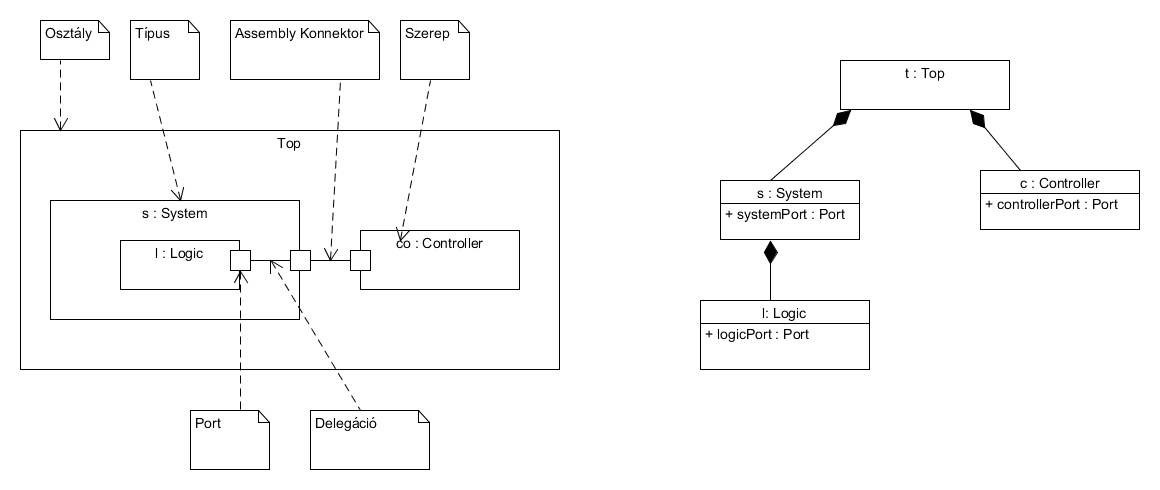
\includegraphics[scale=0.8]{composit_stuct.png}
\caption{Kompozit diagram elemei}
\end{figure}

\subsection{Akció elemek}
\subsubsection{Üzenet küldés/fogadás}
Interfészportok esetén az elvárt interfész leírja, hogy belülről milyen üzeneteket tudunk küldeni a portnak, mely a külvilág felé áramlik tovább, ezt nevezzük portra való üzenetküldésnek. \\ A szolgáltatott interfész pedig azt mondja meg, milyen üzeneteket tudunk fogadni az adott portról, tehát azt, hogy az osztályon kívülről milyen üzeneteket tudunk fogadni az adott portján. Ezt nevezzük üzenet fogadásnak.
\subsubsection{Connect művelet}
A \textit{connect} művelet alapvetően nem létezik UML-ben, \textit{txtUML}-ben azonban ezt használjuk két port összekötésére a konnektoron keresztül. Ahogy később látni fogjuk, a \textit{CreateLink} műveletet fogjuk használni ugyanerre a célra, mivel a szabvány szerint dinamikusan csak ezen művelet mentén tudunk összekötni két elemet.

\section{A txtUML kompozit elemei}
\subsection{Interfészek megadása}
\begin{lstlisting}
public interface ExampleInterface extends Interface {
  public void reception(ExampleSignal1 signal);
  public void reception(ExampleSignal2 signal);
}
\end{lstlisting}
Ebben az esetben az \textit{ExampleSignal1} és az \textit{ExampleSignal2} eseményeket képes fogadni az \textit{ExampleInterface} a fogadó végpontjain keresztül.
 
\subsection{Portok felvétele}
\begin{lstlisting}
public class ExamplePort extends Port<Interface1,Interface2> {}
\end{lstlisting}
\
Állapotgéppel összekapcsolt portok:
\begin{lstlisting}
@BehaviorPort
public class ExamplePort extends Port<Interface1,Interface2> {}
\end{lstlisting}
Ebben az esetben az \textit{ExamplePort} interfészei az \textit{Interface1} és az \textit{Interface2}


\subsection{Konnektorok}
\subsubsection{Konnektor} 
Mivel a portok kompozíciók szerepei között húzódnak, nézzük meg, hogyan néz ki egy kompozíció leírása:
\begin{lstlisting}
class ExampleComposition extends Composition {
  class a extends ContainerEnd<A> {}
  class b extends End<One<B>> {}
}
\end{lstlisting}
Itt \textit{A} a tartalmazó osztály \textit{a} szereppel van feltöltetve a kompozícióban, aki tartalmaz egy \textit{B} típusú osztályt \textit{b} szereppel.

\subsubsection{Assembly konnektor}

\textit{A}-nak legyen két része: \textit{Comp1.b} egy \textit{B} típusú része és \textit{Comp2.c} egy \textit{C} típusú. Legyen \textit{P} \textit{B}-nek egy portja és \textit{Q} \textit{C}-nek egy portja. Ekkor összeköthetjük \textit{P}-t \textit{b} és \textit{Q} \textit{b} és \textit{c} szerepek mentén egy assembly konnektor segítségével. 

\begin{lstlisting}
public class ExampleConnector extends Connector {
  public class connEnd1 extends One<Comp1.b, B.P> {}
  public class connEnd2 extends One<Comp2.c, C.Q> {}
}
\end{lstlisting}

\subsubsection{Delegációs konnektor}
Ha \textit{Comp3.d} egy\textit{D} típusú része \textit{A}-nak, \textit{A}-nak a szerepe \textit{Comp3.a}, \textit{R} \textit{A}-nak egy portja, \textit{S} \textit{D}-nek egy portja, akkor egy delegációs konnektor \textit{R} és \textit{S} között a következőképpen nézhet ki:
\begin{lstlisting}
public class ExampleDelegation extends Delegation {
  public class connEnd1 extends One<Comp3.a, A.R> {}
  public class connEnd2 extends One<Comp3.d, D.S> {}
}
\end{lstlisting}

\subsubsection{Átmenetek kibővítése}
Az az állapotgépek átmeneteinek  \textit{Trigger}-ének megadhatunk egy \textit{port} dimenziót, mely azt mondja meg, hogy a \textit{value} értéken szereplő üzenetnek melyik port legyen a forrása, hogy az átmenet végrehajtódjon.
\begin{lstlisting}
@From(State1.class) @To(State2.class)
@Trigger(port = ExamplePort.class, value = ExampleSignal.class)
class ExampleTransition extends Transition {}
\end{lstlisting}

Ez esetben, ha \textit{State1}-ben vagyunk, és az állapotgépnek küldünk egy  \textit{ExampleSignal}-t, akkor, ha ennek forrása a \textit{ExamplePort}, átlépünk a \textit{State2} állapotba.

\chapter*{2. Áttekintés}
\stepcounter{chapter}
\section{Szabványok és keretrendszerek áttekintése}
\subsection{fUML - ALF}
A Foundational UML (fUML) \cite{fmul} egy Object Managment Group (OMG) által specifikált végrehajtható UML szabvány, 
melynek szöveges akciónyelvi szintaxisát az ALF (Action Language for Foundational UML) \cite{alf} definiálja.
Mivel ALF az UML szabvány egy részhalmazán alapszik, így az akciónyelvi elemekhez és a strukturális elemekhez (osztály, asszociációk)  széleskörű támogatást nyújt, de az állapotgépekhez vagy a kompozíciókhoz nem definiál szintaxist.

\subsection{PSCS szabvány}
A  Precise Semantics of UML Composite Structures (PSCS)  szabvány \cite{pscs} szintén az OMG által specifikált UML szabvány, mely kiegészítve az fUML szabványt, a kompozit struktúrák elemeihez definiál szemantikát. Ebben található meg többek között az osztályok, interfészek pontos szerepeinek leírása a kompozit struktúrákban, valamint a portok, konnektorok és ahhoz kapcsolódó akciókódok szemantikája. A PSCS szabvány szorosan kapcsolódik a \ref{reprezentation} fejezethez, melyben megvizsgáljuk az egyes kompozit elemek UML szabványát a megfelelő modell létrehozásához, valamint a kódgenerálás szemantikájához.

\subsection{Umple}
Az Umple \cite{umple} szöveges alapú modellezőeszköz támogatja a kompozit struktúrák leírását. Itt a portok egyszerű adattagonként jelennek meg, melyekhez úgynevezett aktivátor metódusokat rendelhetünk, melynek hatása az attribútum változásakor érvényesül. A megváltozott állapot kihat a kapcsolatban álló portokra is, a konnektor másik végén álló portok állapota is megváltozik, melyre szintén egy aktivátor függvény segítségével reagálhatunk. A konnektorok pedig egyszerűen portok egymáshoz kötésével jelennek meg (\textit{binding}), konnektor struktúrák és interfész kompatibilitási problémák nélkül. Ezzel szemben a \textit{txtUML}-ben interfészportokat adhatunk meg elvárt és szolgáltatott interfésszel, egyszerű attribútumokat nem, aktivátorok helyett pedig az állapotgép átmenetei vannak kiegészítve a portok dimenziójával. Az Umple nem foglalkozik a szabványos UML2-es reprezentációval, a C++ kódot közvetlen a modell szövege alapján állítja elő. Valamint saját akciónyelvvel sem rendelkezik, hanem azt a célnyelvben adhatjuk meg. \\

Előnyei:
\begin{itemize}
\item Online eszközként is elérhető, nem szükséges hozzá semmit telepíteni.
\item Letisztult, jól definiált szöveges szintaxisa van, beleértve a portokat is.
\item Tartalmaz kódgenerálást.
\end{itemize}
Hátrányai:
\begin{itemize}
\item Nem generál egy szabványos UML modellt a kódgenerálás előtt, közvetlen a szövegre építkezik.
\item A portokat egyszerű adattagként képzi le a feltípusozás alapján, nem lehet megadni szolgáltatott és elvárt interfészeket.
\item Nincs saját akciónyelve.
\item Nincs lehetőség testre szabni az üzenetküldés implementációját a porton keresztül, nincs konfigurációs leírás.
\end{itemize}

\subsection{StartUML}
A StartUML  támogatja a kompozit diagramok létrehozását, így a portokat, konnektorokat és interfészeket is. Vizuális modellezőeszköz, a létrehozott diagramokból C++ kódot tudunk exportálni. A Portok vázát exportálja, ahogy az interfészeket is, de primitív szinten, a portok feltípusozása után egy adattagként generálja hozzá az osztályhoz. A konnektorokat már nem exportálja, ahogy a portokhoz kapcsolódó műveleteket sem. \\
Előnyei:
\begin{itemize}
\item Az UML szabványos elemeivel dolgozik
\item Különböző kiterjesztések révén tartalmaz kódgenerálást
\end{itemize}
Hátrányai:
\begin{itemize}
\item Az eszköz mellett meg kell ismerni precízen az UML szabványos elemeit is, hogy fel tudjuk tölteni az elemek tulajdonságait
\item A kódgenerálás csak a vázra terjed ki, mely tartalmazza a portokra, de az azokkal való műveleteket már nem.
\item Nehézkes, vizuális használat, az elemeket szabadon létrehozhatjuk, és könnyen nem szabványos modellt generálhatunk, míg a txtUML exportja a szabványos modellt exportálás révén hozza létre, így kisebb lehetőségünk van hibázni.
\end{itemize}

\subsection{BridgePoint UML}
A StartUML-hez hasonlóan az UML szabványos elemeiből építhetünk fel vizuálisan egy szabványos UML diagramot, melyet kiegészíthetünk akár nem szabványos elemekkel is. Azonban nem tudunk osztályok között portokkal kommunikálni, csak komponensek között (melyről a \ref{class} fejezetben azt mondtuk, hogy egy kifejezetten speciális elem az UML-ben), így ez a megoldás nem elég általános. Portot, illetve konnektort önmagában nem tudunk felvenni, az interfészek segítségével tudunk egy kapcsolatot húzni két komponens között, mely leképződik egy porttá és konnektorrá. Hasonlóan a StartUML-hez, az akciókat aktivitás node-ok révén kézzel kell összerakni, így nehéz szabványos port műveleteket létrehozni. Összességében a BridgePoint-ról \cite{bridge} is elmondható, hogy kezdetlegesen támogatja a portokkal történő kommunikációt, az ezzel kapcsolatos részei eltérnek a szabványos UML-től, így a kódgenerálás támogatása ellenére nehéz érdemben kompozit elemek kódgenerálási stratégiájáról beszélni. 

\section{Összefoglalás}
Összességében az figyelhető meg az egyes exportálási módok között, hogy a portokat mindig valamilyen primitív feltípusozott adattagként exportáljuk. A másik lehetőségünk, melyet mi is követni fogunk, az interfészportokat összetett típusként exportálni, melyben benne van a szolgáltatott és elvárt interfész. Portok összekapcsolásának, a portokon történő kommunikáció végrehajtási szemantikájával pedig nem mindegyik keretrendszer foglalkozik, még ha részben támogatja is a portok exportálását. Ennek oka a szabvány nehezen érthetőségében és hiányosságában keresendő. Mindebből az figyelhető meg, hogy egy viszonylag új területről beszélünk, melyben egy teljes körű támogatás és elemzés referencia értékű lehet későbbi megoldások, fejlesztések számára. A diplomamunka elemez több különböző, teljes körű megoldást a portok és interfészek C++ nyelvre történő exportáláshoz, mely magában foglalja a szabványos UML modell létrehozását egy jól definiált leírónyelv alapján.

\chapter*{3. Reprezentációs lehetőségek} \label{reprezentation}
\stepcounter{chapter}
\section{A megfelelő reprezentációk megtalálása}
Az eddig leírtakból kiderült, hogy a szabványos reprezentáció megtalálásával is problémákba ütközünk, mely a fellelhető irodalomból és eszközökből is csak nehezen derül ki, így kitérünk ezek ismertetésére is. A C++ reprezentációhoz pedig egy saját port könyvtárat és generálási módszert választunk, mely a fellelhető módszerek finomításából és több különböző ötlet elemzésének alapján hozunk létre. \\

A továbbiakban a következő elemek reprezentációjával foglalkozunk:
\begin{itemize}
\item Interfészek
\item Portok és üzenet küldés/fogadás művelet
\item Konnektorok és connect művelet
\end{itemize}

\section{Portok reprezentálása}

\subsection{UML-ben}
A portok reprezentálása értelemszerű, egy speciális \textit{Property}-t kell felvenni az osztályon belül. Amit fontos megemlíteni, hogy a szolgáltatott interfész segítségével fogjuk feltípusozni. 


\subsubsection{Szemléltetés osztálydiagrammal}
A 3.1-es diagramon láthatjuk, hogy a port leszármazik a szolgáltatott interfészből, megvalósítva azt, és az osztály pedig tartalmazza a portot.

\begin{figure}[H]
\begin{center}
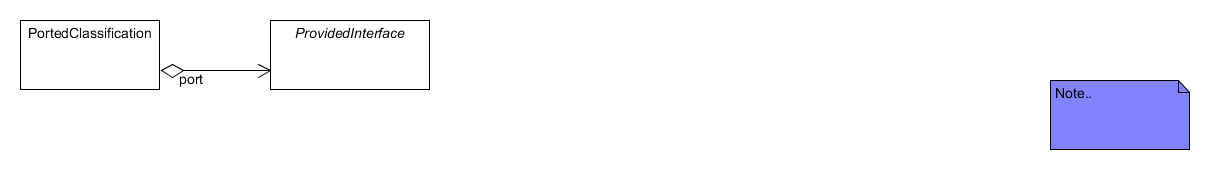
\includegraphics[scale=0.8]{uml_port_class.png}
\end{center}
\caption{Port UML megvalósításának szemléltetése osztálydiagramon}
\end{figure}

\subsubsection{Szemléltetés komponens diagrammal}
Az 3.2-es ábrán egy osztály látható, mely tartalmaz egy portot, melyet a kompozit struktúrákon egy négyzet jelöl. Nincs kapcsolatban másik elemmel, de van egy kapcsolódási pontja, melyet a kör jelöl. \\
\begin{figure}[H]
\begin{center}
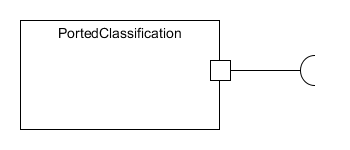
\includegraphics[scale=0.7]{uml_port_comp.png}
\end{center}
\caption{Port UML megvalósításának szemléltetése kompozit diagramon}
\end{figure}

\subsection{C++-ban} \label{cpp_gen_port}
A portokat C++ osztályok adattagjaiként reprezentáljuk. Hasonlóan a \textit{txtUML} Java szintaxisához, felveszünk egy \textit{Port} típust, melyet paraméterezhetünk az interfészek típusával. A \ref{inf} fejezetben részletesen beszélünk arról, hogyan valósítunk meg egy interfész portot C++-ban, és miért erre a szintaxisra esett a választásunk. 

\section{Portokra való üzenetküldés/fogadás reprezentálása} \label{message}
\subsection{UML-ben}

\subsubsection{Üzenetküldés}
A  \textit{SendObjectAction} két paraméterből áll, egy célobjektumból és egy üzenetből.
A célobjektum valamilyen \textit{InputPin}, vagyis valamilyen akciónak az eredménye.
Mivel a port egy strukturális elem, így a referenciáját egy \textit{ReadStructuralFeatureAction} akcióval megszerezhetjük. A megoldást a 3.3-as ábrán szemléltetjük.
\begin{itemize}
\item Könnyű reprezentálni, illeszkedik a modellfordító elvébe, aki feltételezi, hogy
egy \textit{send} akciónak van egy célobjektuma, ahova az üzenetet kell küldeni. Ez a célobjektum ilyenkor maga a port lesz, és nem az azt tartalmazó osztály.
\item Nem kell extra logikát beiktatni a C++ fordítóba az üzenetküldés terén.
\item Szintaktikailag könnyen kivitelezhető, azonban a \textit{PSCS} szabvány nem ír róla semmit, mi lesz a szemantikája egy ilyen konstrukciónak.
\end{itemize}

\begin{figure}[H]
\begin{center}
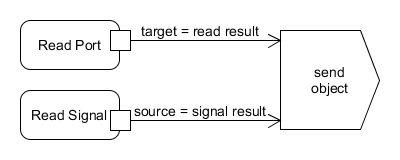
\includegraphics[scale=0.8]{send_uml.png}
\end{center}
\caption{Üzenetküldés a portnak \textit{SendObject} akcióval úgy, hogy a port a célobjektum}
\end{figure} 


A \textit{PSCS} szabvány definiálja, hogy szintaktikailag hogyan néz ki egy üzenetküldése, illetve fogadása porton keresztül, és mi lesz ennek a pontos szemantikája. \\
Ha egy osztály példánynak a portján keresztül szeretnénk üzenetet küldeni, akkor a \textit{SendObjectAction}-nak az \textit{OnPort} adattagját használhatjuk a szabvány szerint.  Az \textit{OnPort} adattag egy \textit{Port} típusú referencia adattag, melyet ha nem adunk meg, akkor az üzenetet a célobjektumnak küldjük el, és az objektumnak való üzenetküldés szemantikája nem változik.  Azonban, ha ez ki van töltve, akkor az objektumnak a portján keresztül továbbítunk üzenetet. Ennek szemantikája pedig attól függ, hogy milyen kontextusban hajtottuk végre az akciót. \\

Ha az akció környezete szerint az üzenetküldés kezdeményezője az az objektum, akinek a portjára üzenetet szeretnénk küldeni, vagyis megegyezik a \textit{target} referenciával, akkor üzenetküldésről beszélhetünk (\textit{send} művelet). \\
Ha a \textit{SendObjectAction} kezdeményezése a célobjektumon kívülről történt, akkor pedig üzenet fogadásról beszélhetünk (\textit{receive} művelet). \\
 
\begin{figure}[H]
\begin{center}
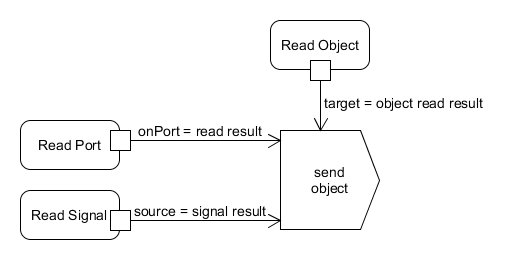
\includegraphics[scale=0.7]{receive_uml.png}
\end{center}
\caption{Üzenetküldés/fogadás port felhasználásával \textit{SendObject} akcióval a \textit{OnPort} referencia kitöltésével}
\end{figure} 

\subsection{C++-ban}
C++ exportálás során az üzenetküldés fordítását kell átdolgozni, figyelembe kell venni az \textit{OnPort} referenciát, valamint az üzenetküldés kezdeményezőjét a szemantikának megfelelően. \textit{txtUML}-ben az üzenet fogadás nem megvalósított, de a kódgenerátor felkészíthető rá.

\subsubsection{Üzenetküldés}
Az üzenetküldés C++-ban egy \textit{send} műveletre fog fordulni, melynek első paramétere a port, a második pedig a küldendő üzenet. Az üzenetküldés szintaxisa így lesz a legtisztább, így ennek a szemantikáját érdemes megvizsgálni. A \textit{send} művelet azt jelenti, hogy a portra teszünk egy üzenetet, melyet továbbítunk egy másik egység felé konnektoron keresztül. Ennek szemantikájával a \ref{connect} fejezetben foglalkozunk részletesen.

\subsubsection{Üzenetfogadás}
Valahogyan ki kell fejeznünk azt is, ha egy üzenetet nem a külvilág felé delegálunk, hanem a külvilág felől érkezett egy üzenet a portra, melyet fel kell dolgoznunk állapotgéppel összekapcsolt portok esetén, vagy tovább delegálunk a belső komponensek felé. Erre két lehetőségünk van:
\begin{enumerate}
\item Egy teljesen új függvényt vezetünk be (nevezzük ezt \textit{receive}-nek)
\item Paraméterezzük a \textit{send} függvényünket egy környezet változóval, melyben megadhatjuk az üzenetküldés kontextusát a PSCS szabványhoz hasonlóan.
\end{enumerate} 
Előbbi megoldás azonban tisztább, jobban érthető a felhasználó számára, valamint a szolgáltatott és elvárt interfészek kifejezésénél is előnyösebb lesz. (\ref{inf}) \\

A 3.5-ös ábra azt szemlélteti, hogy melyik akciót kell lefuttatni attól függően, hogy a portra való üzenetküldés milyen kontextusban történt, melyik irányból. \\

\begin{figure}[H]
\begin{center}
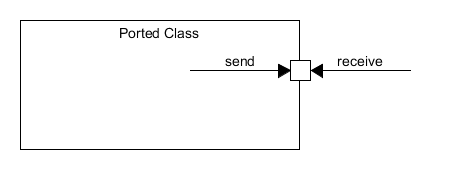
\includegraphics[scale=0.8]{send_rec.png}
\end{center}
\caption{Üzenetküldés/fogadás kontextusa}
\end{figure} 

\subsubsection{Üzenetfogadás állapotgéppel összekapcsolt portok esetén}
Az állapotgéppel összekapcsolt portok többféleképpen használhatók kommunikációra, de minden esetben egyfajta ravaszként működik a rajtuk történő állapotváltozás (amikor egy állapotgéppel összekapcsolt port értéke megváltozik, pl. üzenet érkezik rá). A port adattag értéke reprezentálja az üzenetet. Ennek megfelelően általánosságban kétféle megoldás létezik a portokon történő kommunikáció megvalósítására:
\begin{itemize}
\item Hasonlóan az események feldolgozásához, úgy a portokon történő üzenetfogadást is átmeneti függvényekkel dolgozzuk fel. Ez esetben nem érdekes számunka a port állapota, az üzenet az objektum üzenetsorába kerül be, mely majd feldolgozásra kerül hasonlóan, mint egy normál üzenet.  \\

\begin{figure}[H]
\begin{center}
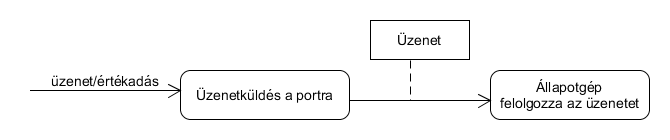
\includegraphics[scale=0.6]{port_actfun.png}
\end{center}
\caption{Portról fogadott üzenet feldolgozása állapotgéppel}
\end{figure} 

\item Külön aktivátor (figyelő) függvényeket valósítunk meg az osztályon belül az egyes portokra, melyek a portok állapotváltozásakor aktiválódnak. Ez esetben számít a portnak az állapota, mivel az reprezentálja magát az üzenetet. Ennek megfelelően máshogy dolgozzuk fel, mint a többi üzenetküldést. Interfészportok esetén a port tartalmazza a neki küldött üzenetet, az reprezentálja az állapotát, primitív esetben pedig a port értéke szolgál erre. \\


\begin{figure}[H]
\begin{center}
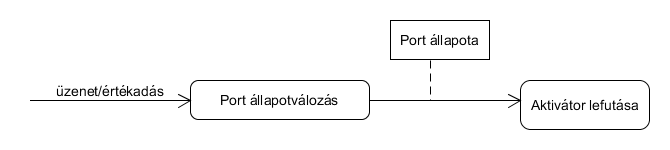
\includegraphics[scale=0.6]{port_sendm.png}
\end{center}
\caption{Portról fogadott üzenet feldolgozása aktivátor függvénnyel}
\end{figure} 

\end{itemize}

A mi esetünkben az előbbi megoldás tűnt kézenfekvőnek, mivel az könnyen adaptálható a meglévő generálási szabályok közé, valamint a forrásnyelv is ezt a konvenciót követi. A \ref{comm} fejezetben kitérünk arra, hogy az osztály állapotgépe pontosan hogyan dolgozza fel az adott üzenetet. Nem-állapotgéppel összekapcsol portok esetén pedig továbbítanunk kell az üzenetet a belső port felé, ilyenkor az állapotgépnek nem kell reagálnia rá. Ezzel a \ref{connect} fejezetben részlesen foglalkozunk.

\section{Interfészek reprezentálása interfészportok esetén} \label{inf}
\subsection{UML-ben}
Az interfészeket UML-ben értelemszerűen reprezentáljuk, annyiban különböznek csak az osztályoktól, hogy megadhatunk neki fogadási műveleteket, ún. fogadó végpontokat. Egy-egy végpont egy olyan metódusnak felel meg, melynek pontosan egy paramétere van, egy \textit{Signal} típusú paraméter. 

\subsection{C++-ban}
C++-ban számos lehetőségünk van kifejezni egy UML interfészt.
\subsubsection{Nincs interfész}
Egy lehetséges megoldás az is, ha nem vesszük figyelembe a szolgáltatott és elvárt interfészeket akkor, mikor egy adott portot manipulálunk, üzenetet küldünk rá. Ekkor a forrásnyelv validációja hivatott kiszűrni az ilyen nem helyes üzenetküldéseket, hivatkozásokat. \\
Előnyök:
\begin{itemize}
\item Kódgenerálás szempontjából nagyon triviális megoldás, egyáltalán nem szükséges foglalkozni az interfészek az interfészek exportálásával C++-ban.
\item Alacsony szintű, hatékonysági kérdésekben a legjobb megoldás, mivel se futási idejű, se fordítási idejű validáció nincs. 
\end{itemize}
Hátrányok:
\begin{itemize}
\item Külső osztályok, portok esetén a felhasználó sem tud felvenni interfészeket, ilyenkor már nem hagyatkozhatunk a forrásnyelv validációjára, könnyen hibázhatunk.
\item Ha nem is vezetünk be új komponenst, külső kommunikáció esetén tetszőleges üzenetet küldhetünk a portra, ami szintén hibás lehet.
\item A generált kód kevésbé lesz érthető.
\item Az interfészeket sehol máshol sem tudjuk felhasználni, osztályok sem tudják megvalósítani őket, mely szintén a modellel való kommunikációban jelent hátrányt. 
\end{itemize}

\subsubsection{Van interfész}
Ezen belül meg kell vizsgálni az interfész port szintaxisát, valamint a mögöttes végrehajtási szemantikát, illetve magának az interfésznek a leírási módjait. \\
Ahogy azt korábban írtuk, a port típusa az UML-ben a szolgáltatott interfész, ezért kézenfekvő megoldás lenne felvenni egy olyan adattagot, melynek ez az interfész a típusa. Ennek azonban több hátránya is van, sokkal nehezebben tudjuk kifejezni, milyen elvárt interfésze van a portnak, valamint nem tudjuk kifejezni a port típuson belül az üzenetküldés végrehajtási szemantikáját sem, valamilyen külső implementációra kényszerülünk. Ezáltal bonyolítjuk a megvalósítást, veszítünk az absztrakcióból, de a hatékonyságot nem növeljük. 
Így a másik lehetőségünk bevezetni a \textit{Port} típust, melynek sablon paramétere a szolgáltatott és elvárt interfész, ahogy azt a 3.8-as ábrán is láthatjuk. \\

\begin{figure}[H]
\begin{center}
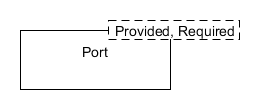
\includegraphics[scale=0.7]{port_class.png}
\end{center}
\caption{Port az interfészek sablonparamétereivel}
\end{figure} 


Ezek után technikailag többféle lehetőségünk van megvalósítani a validációt: \\
\begin{enumerate}

\item Generáljunk egy üres osztályt az interfészekből, majd a szignálok származzanak le aszerint, hogy melyik interfész fogadó műveletei között vannak benne: \\
PL: UML interfész neve: \textit{PingPongInterface}, a fogadó végpontjai pedig a következő szignálokat fogadják: \textit{Ping}, \textit{Pong} \\
Majd a portnak legyen egy \textit{send} művelete, ami az elvárt interfész alá sorolt szignálokat várja, vagyis olyan szignálokat, melyek implementálják a megfelelő interfészt.
Mindezzel fordítási időben biztosítjuk, hogy ne adhassunk át olyan szignált, melyet nem soroltunk az elvárt interfész szignáljai közé. Hasonlóan, a \textit{receive} művelet olyan szignálokat vár, melyek leszármazottjai a szolgáltatott interfésznek (lásd 3.9-es ábra). \\

\begin{figure}[H]
\begin{center}
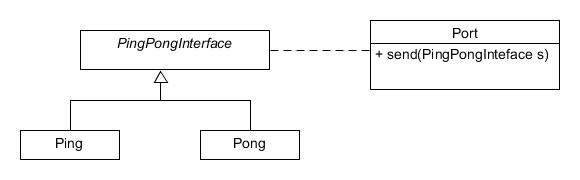
\includegraphics[scale=0.7]{inf_ver1.png} \\
\end{center}
\caption{Szignálok csoportosítása leszármazással}
\end{figure}

Előnyök:
\begin{itemize}
\item Egyszerű megvalósítás, kevés extra kód generálásra van szükség hozzá, az interfészek lényegében csak üres, csoportosító osztályok.
\item Egyetlen \textit{send} függvénnyel meg lehet oldani a validációt, így a kód a lehető legkisebb lesz, nem lesz redundancia.
\end{itemize}
Hátrányok:
\begin{itemize}
\item Nem általánosított megoldás. Az interfészt bármilyen szereplő használhat, és le is származhat belőle, azonban ezzel erősen portokra korlátozzuk a megoldást, mivel a küldő és fogadó műveletek a portok kódjába vannak beleégetve.
\end{itemize}
\item Ezt a gondolatmenetet folytatva vizsgáljuk meg azt az általános lehetőséget, hogy a \textit{Port} osztály megvalósítja az interfészt. A szintaxis nem változik, továbbra is sablon paraméterként szeretnénk megadni az interfészeket a portban. Mivel most a szignáloknak nincsen interfész őse, így minden egyes fogadási végpont művelethez kelleni fog egy-egy függvény. Mivel az üzenetküldés végrehajtási szemantikája nem változik, így vezessünk be egy általános \textit{sendAny} védett metódust, mely bármilyen szignált képes fogadni, azonban a publikus interfészen nem látható. Ezt a leszármazott osztályban felül tudjuk definiálni az üzenetküldés szemantikájától függően. Amikor a \textit{sendAny} továbbítja az adott portnak a megfelelő szignált, a túloldalon lévő port már csak egy általános eseményt lát, nem tudjuk ellenőrizni a típuskonzisztenciát. Azonban két port összekapcsolásakor tudunk gondoskodni róla, hogy ne köthessünk össze inkonzisztens interfészű portokat (lásd részletesebben a \ref{connect} fejezetben). \\

\begin{figure}[H]
\begin{center}
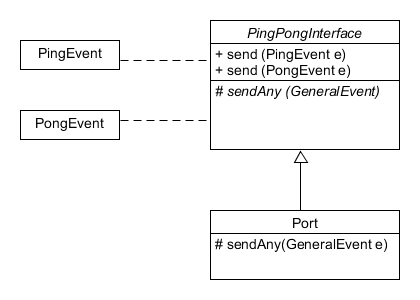
\includegraphics[scale=0.7]{inf_ver2.png} \\
\end{center}
\caption{Szignálok csoportosítása \textit{send} függvényekkel}
\end{figure}


Előnyök:
\begin{itemize}
\item Általános megoldás, az interfészt ténylegesen megvalósítjuk, így ez akár modell osztályokra is kiterjeszthető
\item Funkcionálisan nem különülnek el a \textit{send} függvények egymástól, így a karbantartási idő nem nő
\end{itemize}
Hátrányok:
\begin{itemize}
\item A generált kód mérete azonban jelentősen megnő, mivel több \textit{send} függvény generálásra van szükségünk, melyek csak a várt szignáltípusban különböznek.
\end{itemize}
\item Mint a fentiekből látjuk, az utóbbi megoldásnak egy hátránya van, hogy növeljük az interfész kódját az első megoldáshoz képest. Amíg csak generáljuk az interfészt, addig ez elhanyagolható tényező, azonban, ha kézzel kell hozzáadni a programunkhoz, hogy kiterjesszük a modellel való kommunikációt, már probléma lehet. Megfigyelhetjük, hogy minden interfész implementációja csak abban fog különbözni, hogy különböző szignálokat tudnak fogadni. A C++ sablon metaprogramozási lehetőségeit kihasználva próbáljuk meg az interfész kódját egészen odáig szűkíteni, hogy csak fel kelljen sorolni egy típuslistába, hogy milyen szignálokat tudunk küldeni, illetve fogadni. \\
Cél szintaxis: 
\begin{lstlisting}
using PingPongInf = GeneralInterface<Ping,Pong>
\end{lstlisting}
Ez azt jelentené, hogy a \textit{PingPongInf} egy olyan interfész lenne, amelynek két fogadó művelete van, a \textit{Ping} és a \textit{Pong}.\\
Vizsgáljuk meg a szolgáltatott részt, az elvárt ezzel analóg. Vezessünk be egy olyan sablon \textit{send} függvényt, melynek a sablon paramétere az elküldendő szignál típusa. Ezt látjuk a publikus interfészen, eszerint bármilyen szignállal meg tudjuk hívni az adott függvényt. Azonban a függvény delegálja a hívást egy olyan védett sablon függvénynek, mely bármilyen szignált képes fogadni, és rendelkezik egy logikai sablon paraméterrel: ebben adhatjuk meg, hogy a delegált szignál része-e az interfésznek vagy sem. 
Sablon specializáció segítségével kétféle implementációt adunk ennek a függvénynek: Az igaz ág, mely végrehajtja a szignál küldését, a hamis ág pedig szemantikai fordítási hibára fut, ezzel ellenőrizve fordítási időben, hogy ne adhassunk át olyan eseményt, mely nem része az interfésznek. \\
A kérdés már csak az maradt, hogyan döntjük el egy adott szignálról, hogy része-e az interfésznek. Az egyik lehetőség bevezetni egy sablon osztályt, melynek egy adattagja megmondja, hogy szignálról beszélünk-e, mely paramétere egy fogadási műveletnek. Ezt alapértelmezetten hamisra állítani, és specializálni igaz értékekkel a sablon osztályt a megfelelő szignálokkal. \\
Összefoglalva az eddigieket egy ábrában:
\begin{figure}[H]
\begin{center}
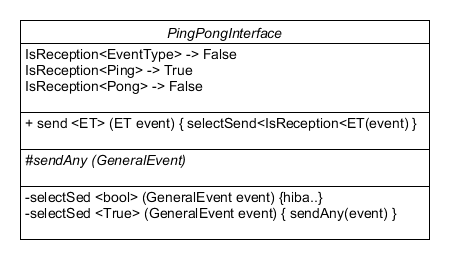
\includegraphics[scale=0.6]{better_inf.png} \\
\end{center}
\caption{Szignálok csoportosítása \textit{IsReception} sablonfügevénnyel}
\end{figure}

Ezzel azonban még nem értük el a kívánt egyszerű szintaxist, de a \textit{send} függvényt legalább nem duplikáltuk fölöslegesen. A \textit{TYPELIST} \cite{typelist} konstrukciót használva viszont eljutunk a cél szintaxisig, ugyanis felsorolhatjuk a megfelelő szignál típusokat egy listában, és elég arra vizsgálnunk, hogy az adott szignál típus része-e a listának.
\end{enumerate}

A legutolsó megoldás tekinthető a legelőnyösebbnek, tartalmazza a második előnyeit, azonban a hátrányait sikerült kiküszöbölni.

\subsection{Szolgáltatott és elvárt interfészek megkülönböztetése}
\subsubsection{UML-ben}
Az UML szabvány szerint egy \textit{konnektor} csak olyan portok között
húzódhat, melynek a szolgáltatott és elvárt interfészei kompatibilisek egymással.
A port egy kommunikációs csomópontot reprezentál, a típusa azonban adattag révén tetszőleges lehet.
A modellosztály számára a port szolgáltatásokat nyújt a szolgáltatott interfész által, így a típusa megfelel a szolgáltatott interfésznek.
A modellosztály azonban kifele továbbít a porton keresztül információkat, az elvárt interfész által.
Húzzunk be egy \textit{Using} relációt a port és az elvárt interfész között, mivel a modellosztály a portot használja üzenetküldésre.
A probléma, hogy a \textit{Using} relációk nem kölcsönösen egyértelműek, ha két portnak ugyanaz a szolgáltatott interfésze, így
érdemes minden portnak egy saját interfészt generálni, amely leszármazottja a szolgáltatott interfésznek. Így minden port típusa egyedi lesz, és a relációk is injektívek lesznek a modellben.
\subsubsection{C++-ban}
Mivel a portra tudunk üzenetet küldeni és fogadni egyaránt, így az interfészeknek két részük lesz, az egyik a fogadó, a másik a küldő műveleteket definiálja. Attól függően, hogy az adott interfészt szolgáltatott vagy elvárt interfésznek adtuk meg, a megfelelő részből fog leszármazni az adott port. A másik lehetőség az lenne, ha nem bontjuk két részre az interfészt, helyette a fogadó végpontok függvényeinek egy plusz paramétere lenne, hogy kívülről vagy belülről küldünk-e üzentet (ahogy azt a \ref{message} bekezdésben felvezettük). Ez esetben abba a problémába ütköznénk, hogy nem tudnánk elkülöníteni a fogadó műveleteket leszármazással aszerint, hogy a port milyen szolgáltatott és elvárt interfésszel rendelkezik. \\

\subsubsection{Interfész kiterjesztett szintaxisa, konkrét példa portok esetén}
\begin{figure}[H]
\begin{center}
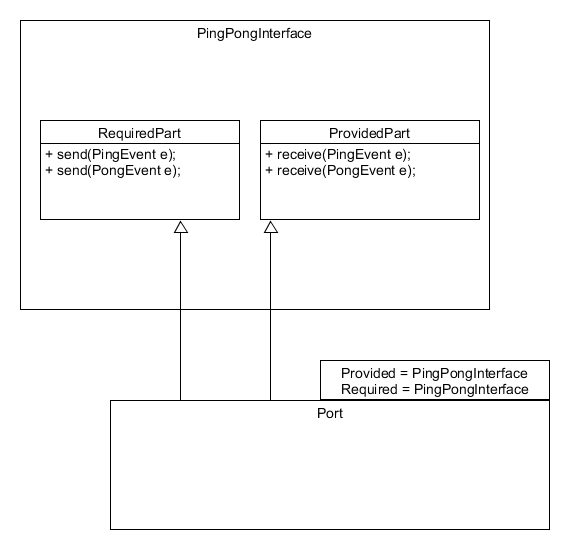
\includegraphics[scale=0.7]{seperate_inf.png} \\
\end{center}
\caption{Interfészek két részre bontva üzenetküldés/fogadás szerint}
\end{figure}

Az 3.12-es ábrán a portnak a szolgáltatott és elvárt interfésze is a \textit{PingPongInterface} lesz. Az interfész maga nem tartalmaz egyetlen fogadó végpontot sem, helyette két különböző részből áll. Az egyik részben az üzenetküldő függvények, a másik részben pedig az üzenetfogadó függvények vannak felsorolva. Ha egy port szolgáltatott interfészének adjuk meg az adott interfészt, akkor az üzenetfogadó résztől (\textit{ProvidedPart}) örökli meg az egyes műveleteket. Ha elvárt interfésznek adjuk meg a \textit{PingPongInterface}-t, akkor pedig a \textit{RequiredPart}-tól örököljük meg az egyes üzenetküldő műveleteket. A konkrét példában azt láthatjuk, hogy a \textit{Port} a \textit{PingPongInterface} fogadó és küldő műveleteit is örökli, mivel az elvárt és szolgáltatott interfésze megegyezik.

\section{Konnektorok, összekapcsolás művelet reprezentálása} \label{connect}
Az interfészeket (\ref{inf}) és portokat már tudjuk exportálni UML-ben, illetve megfelelő C++ reprezentációt is találtunk. A konnektorokat ezek segítségével már ki tudjuk fejezni. \\
Mivel \textit{txtUML}-ben 1-1 kapcsolatokat tudunk csak leírni, így a mi megoldásainkat is erre korlátozzuk. Először megvizsgáljuk, mi lehet a szabványos reprezentáció UML-ben, majd kitérünk a különböző megoldásokra C++-ban. \\
Mielőtt még tovább megyünk, elevenítsük fel, mik is azok a konnektorok és mely részei érdekesek számunkra. A konnektorok egy kompozit struktúrában szerepeket kötnek össze, amik olyan osztályokat fejeznek ki, melyek rendelkeznek porttal. A konnektor egyfajta absztrakciót fejez ki két szereplő portja között, leírja, a szereplő mely két portja kapcsolódik össze, delegációval vagy assembly kapcsolattal vannak-e összekötve. A delegáció szülő-gyerek portok között jöhet lére, ilyenkor egy portra való üzenetküldést delegálunk a túloldalon lévő portra, mely továbbküldi a belső osztály felé, vagy a másik irány esetén a külvilág felé, az osztályon kívülre. \textit{Assembly} összekapcsolás esetén két egyenrangú osztályok portja között jön létre kapcsolat, kölcsönös, oda-vissza kommunikációval. Fontos, hogy szülő-gyerek osztályok között nem lehet assembly kapcsolat, illetve egyenrangú szereplők között delegációs kapcsolat.
\subsubsection{Konnektor reprezentáció UML-ben}
A szabvány szerinti reprezentáció értelemszerű, egy \textit{Connector} UML elemet kell létrehozni, a végpontoknak megadni a kompozíció szereplő portjait, beállítani, hogy \textit{Assembly} vagy \textit{Delegációs} összekapcsolás van-e közöttük. A \textit{Connector} elemnek van egy \textit{Asszociáció} típusa, mivel a szabvány szerint a \textit{Connector} egy \textit{Asszociáció} egy konkrét realizációja. Hogy mi legyen ez a típus, azzal később foglalkozunk.

\subsubsection{Összekapcsolás művelet reprezentációja UML-ben}
A \textit{connect} akció kifejezése UML-ben már kevésbé egyértelmű, mivel \textit{connect} akció nem létezik explicit a szabványban. Több lehetőséget is megvizsgáltunk, mire eljutottunk a helyes reprezentációhoz.
\begin{enumerate}
\item Mivel a port adattagok az UML-ben (\textit{Propertyk}) így két portot kölcsönösen értékül adhatunk egymásnak. Ez egy lehetőség arra, hogy kifejezzük UML-ben az összekapcsoló műveletet, szabványos modell keletkezik, de mégsem ez a helyes szabványa portok összekapcsolásának. A probléma ugyanis az, hogy bármilyen két portot összekapcsolhatunk, konkrét konnektor realizáció nélkül.
\item A \textit{PSCS} szabvány szerint, ha egy operáció egy konstruktor hívásnak felel meg (\textit{Create} sztereotípiával van ellátva), és nem adunk meg hozzá konkrét metódustörzset, mint akciót, akkor az osztály kompozit struktúráját valamilyen alapértelmezett konstrukciós stratégia mentén fogja létrehozni (Ezt nevezi a szabvány \textit{DefaultConstruction}-nek). Mivel a \textit{Connector} egy asszociáció példány, így már egy konkrét, létrejött kapcsolatról beszélhetünk, az alapértelmezett konstrukciós stratégia pedig megmondhatja, hogyan kell összekötni a portokat. Ebből adódóan a kompozíció struktúrájából következtethetünk az összekapcsolt portokra. Azonban ez megszorításokkal járna, ha például egy szülőnek két azonos típusú gyereke van, de csak az egyikkel szeretne delegáció révén kommunikálni, nem lehet hozzá kötni mindkét gyerek porthoz a szülő portját.  \\

\begin{figure}[H]
\begin{center}
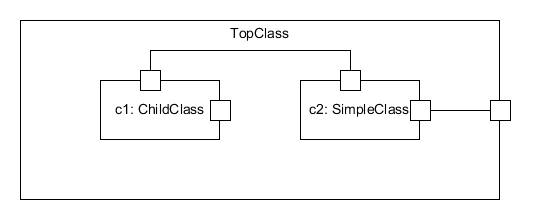
\includegraphics[scale=0.8]{preconnect_problem.png}
\end{center}
\caption{Probléma a statikus összekapcsolással}
\end{figure}


\item Nem maradt más lehetőség, mint a dinamikus összekapcsolás, tehát meg kell mondani egy konkrét metódusban, hogyan inicializáljunk fel egy struktúrát. Szintaktikailag sincs már más lehetőség, mint a \textit{CreateLinkAction} használata, melyet a \textit{PSCS} szabvány definíciója is kimond. Ehhez két dologra van szükség: végpontokra (\textit{LinkEndData}), valamint arra az asszociációra, melyet használni szeretnénk az összekapcsoláshoz. Az asszociáció végpontok egyértelműek, felhasználhatjuk a konnektor végpontjait. Mint korábban láttuk, a konnektorok fel vannak típusozva egy \textit{Association} típussal. Értelemszerű lenne ezt fölhasználni az összekapcsoláshoz, a kérdés csak az, mi legyen ez az asszociáció. A szabvány biztosít nekünk egy alapértelmezett asszociációt (\textit{GenericAssociation}), melyet használhatunk abban az esetben, ha a konnektornak nincs típusa. Arra is van lehetőségünk, hogy saját asszociációt generáljunk a modellbe. Asszociáció típusok között húzható, a port önmagában nem típus, hanem egy adattag, de ennek révén rendelkeznek típussal, a szolgáltatott interfészének a típusával. Vegyük két port interfészét, nevezzük ezeket \textit{t1}-nek, illetve \textit{t2}-nek.  Megtehetjük, hogy generálunk \textit{t1} és \textit{t2} között egy \textit{a1} asszociációt, melyet a konnektor realizál a portok összekapcsolásával. Így a \textit{CreateLinkAction}-be be tudjuk tenni asszociációként az \textit{a1}-et, mint a konnektor típusát, ami mentén összekapcsolunk, nem kell használnunk a \textit{GenericAssociation}-t. Ezzel egy szabványos UML-t generálunk, és a konnektorokat sem hagyjuk figyelmen kívül két port összekapcsolásánál. \\

\begin{figure}[H]
\begin{center}
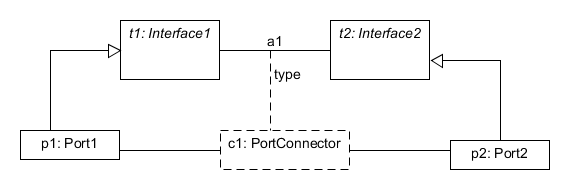
\includegraphics[scale=0.8]{connect_type.png}
\end{center}
\caption{Konnektor típusának megadása}
\end{figure}

Az 3.14-es ábrán látható, hogy a \textit{p1} és \textit{p2} portnak a típusa az \textit{t1} és \textit{t2} interfészből származik, melyek között húzódik egy \textit{a1} asszociáció. Ezek után a \textit{c1} konnektor \textit{type} referenciájába az \textit{a1} asszociáció kerül bele. 
\end{enumerate}

\subsection{Összekapcsolt portok reprezentációja C++-ban} \label{conn_cpp}
A szabvány szemantikája szerint, amikor egy üzenet küldünk a \textit{send} művelettel egy adott portra, annak továbbítania kell ezt a vele kapcsolatban álló port felé. Ehhez egy referenciát kell tárolni a kapcsolt portra. Ezt alapvetően kétféleképpen érthetjük el:\\
\begin{enumerate}
\item Egy globális adatszerkezetben, például egy asszociatív tömbben megmondjuk, melyik porthoz ki kapcsolódik. Ennek előnye, hogy a port kódja független marad a kapcsolatoktól, nem kell belekódolni a kapcsolatok kifejezéséhez új adattagokat.
Hátránya az, hogy egy párhuzamos környezetben egy globális adatszerkezetet kell manipulálni, mely sok szinkronizációt igényel, minek következtében csökken a hatékonyság.
\item A másik lehetőségünk, hogy a port kódjában közvetlen referenciát tárolunk a kapcsolt portra. Mivel az nem lesz érdekes az üzenetküldés szemantikájában, hogy pontosan melyik konnektoron keresztül kapcsolódnak az adott portok egymáshoz (annak típusa azonban számítani fog), és csak 1-1 kapcsolatot valósítunk meg, így a port kódját nem kell a modell alapján generálnunk, nem fog bővülni, és hatékonyabb megoldást érhetünk el szekvenciális környezetben is, mint a globális adatszerkezettel. 
\end{enumerate}

Az üzenetküldés szemantikájához már megvan a referenciánk, azonban ez önmagában még nem elég. Figyelembe kell vennünk azt is, hogy milyen típusú konnektoron keresztül kapcsolódtak az adott portok. Másképp kell átadni az üzenetet, ha Delegációról van szó, és másképp, ha \textit{Assembly} kapcsolatról. Delegációs kapcsolat esetén, ha üzenetet küldünk kívülről egy adott portra (\textit{send} művelet), akkor a szemantika szerint az üzenetküldésünk ekvivalens a kapcsolt portra való belső üzenetküldéssel. \textit{Assembly} kapcsolat esetén azonban ez az üzenetküldés a kapcsolt portra való külső üzenetküldéssel lesz ekvivalens (\textit{receive} művelet).
Így tudnunk kell, hogy a referenciánk milyen kapcsolatban áll a portunkkal. Két lehetőségünk van ennek kifejezésére, a választás nem egyértelmű:
\begin{enumerate}
\item Virtualizáció használata, \textit{Port} típusú referencia helyett \textit{Connection} típusú referencia, melynek absztrakt művelete eldönti, a kapcsolt port melyik műveletét kell meghívni. Ez egy tisztább implementáció, azonban a virtualizáció nem elég hatékony.

\begin{figure}[H]
\begin{center}
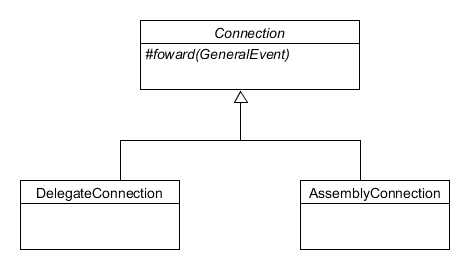
\includegraphics[scale=0.65]{connection.png} \\
\end{center}
\caption{\textit{Connection} absztrakt osztály használata}
\end{figure}

\item Delegáció jelző használata: Marad a \textit{Port} típusú referencia, maga a port dönti el, melyik művelet hívására van szükség a jelző alapján. Ez a megoldás kevésbé letisztult, de hatékonyabb. \\
\begin{figure}[H]
\begin{center}
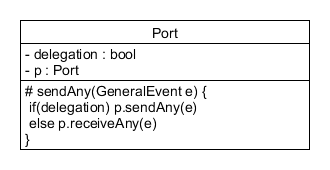
\includegraphics[scale=0.9]{connection_with_flag.png} \\
\end{center}
\caption{\textit{Delegatiom flag} használata}
\end{figure}

\end{enumerate}


Hasonlóan az interfészek megoldásához, itt is az a megoldás lenne hatékonyabb, mely mindkét megoldás előnyeit kombinálja, tehát nem veszítünk a hatékonyságból, de megtartjuk a tiszta implementációt. Ha dolgozhatnánk leszármazással, ugyanakkor nem kéne virtualizációt használni. Erre egy kézenfekvő megoldás az lenne, ha a leszármazáskor megadnánk az interfésznek sablon paraméterben, ki a leszármazottja. \\
Cél szintaxis:
\begin{lstlisting}
class DelegateConnection : public Connection<DelegateConnection>
\end{lstlisting}

Majd definiálnánk a speciális implementációkat, az interfész implementáció pedig statikus konverzióval a specializált \textit{Connection} osztályra konvertálná önmagát, és meghívná a megfelelő műveletet. Ehhez fordítási időben tudni kell, hogy egy adott porthoz milyen típusú kapcsolaton keresztül fog létrejönni a referencia (\textit{Assembly} vagy \textit{Delegáció}). \\ 
A portokat akkor kapcsoljuk össze, mikor létrehozzuk a rendszer struktúráját. Minden port 1-1 kapcsolattal kapcsolódik egymáshoz. Ami azt jelenti, hogy egy állapotgéppel összekapcsolt port esetén egy referenciánk lesz egy másik portra, melyet valamilyen ismert kapcsolaton keresztül kötünk majd hozzá. Általános port esetén pedig két referenciánk lesz, az egyik biztosan egy delegáció, a másik pedig ugyanazon az érvek mentén ismert, amit az előbb tárgyaltunk. Ebből következtetve úgy tűnik, hogy ha a pontos összekapcsolást nem is ismerjük, de a potenciális összekapcsolások típusait igen, akkor fordítási időben el tudjuk dönteni egy adott kapcsolatról, milyen típusú. Az is lehetséges, hogy egy félkész, vagy hibás modell exportálása esetén egyáltalán nem adunk meg konnektort két port között. Ilyenkor exportálási hibát nem célszerű adni, mivel lehetséges, hogy a felhasználót tudatosan érdekel egy ilyen modellnek a C++ kódja, helyette inkább bevezetünk egy \textit{NoConnection} típusú leszármazást, melynek műveleteinek szemantikája megegyezik az üres utasítással. Akár sablon specializációval is dolgozhatunk, mely azért is lesz előnyös, mert a \textit{Connection} ősosztályban általánosan tárolunk egy port referenciát, melyeket a leszármazottak megörökölnek, így ezt az adattagot megspórolhatnánk.

\subsubsection{Megoldás szemléltetése}
\begin{enumerate}
\item \textit{NoConnection} leszármazással: \\

\begin{figure}[H]
\begin{center}
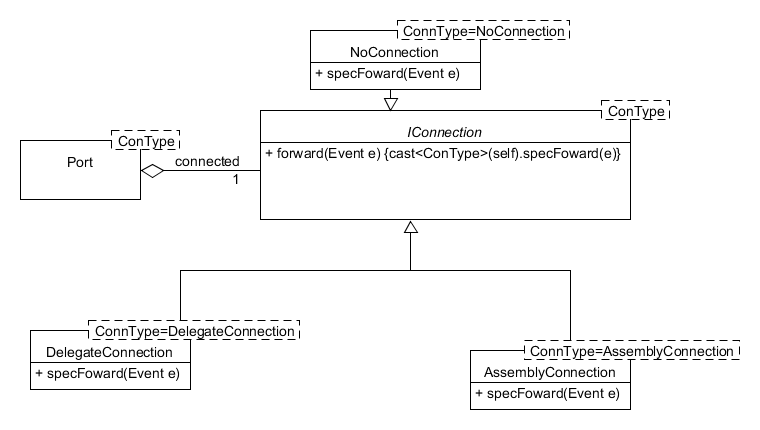
\includegraphics[scale=0.6]{extended_connection.png}
\end{center}
\caption{\textit{Connection} osztály leszármazott sablonparaméterrel}
\end{figure}

Ebben az esetben a \textit{NoConnection} osztály leszármazik az \textit{IConenction}-ből, így tartalmazza a \textit{Port} típusú \textit{connected} referenciát.
\item \textit{NoConnection} specializációval: \\

\begin{figure}[H]
\begin{center}
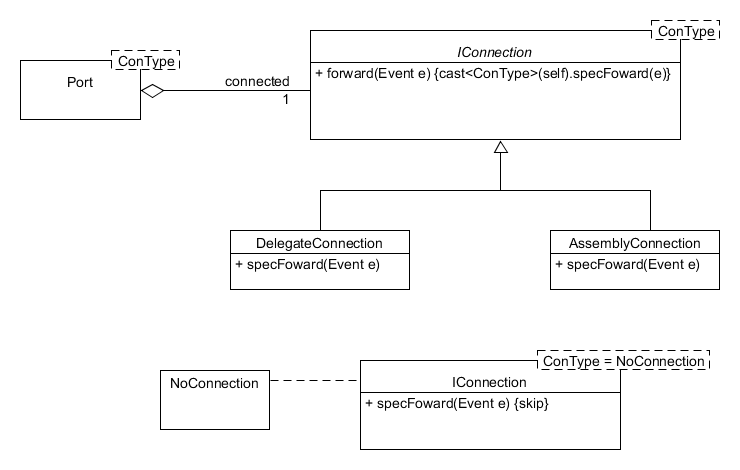
\includegraphics[scale=0.6]{extended_connection_spec.png}
\end{center}
\caption{\textit{Connection} osztály leszármazott sablonparaméterrel, \textit{NoConnection} specializációval}
\end{figure}

Ebben az esetben a \textit{NoConnection} osztály csak egy szereposztály, mellyel specializáljuk az \textit{IConnection} osztályunkat, így elhagyhatjuk belőle a \textit{Port} típusú referenciát is.
\end{enumerate}

\subsection{Különböző port típusok megvalósítása C++-ban}
Az üzenetküldés megvalósítása után vizsgáljuk meg az üzenetfogadás (\textit{receive}) szemantikáját is. A fogadás művelet végrehajtási szemantikája attól függ, hogy állapotgéppel összekapcsolt portról (\textit{BehaviorPort}) beszélünk-e vagy általános portról. Előbbi esetén egy objektum állapotgépéhez futnak be az üzenetek, a másik esetben pedig a szülő komponens portja delegálja az üzenetet a gyerek osztály portjára. Ennek megvalósítására szintén a korábban említett lehetőségeink vannak, a leszármazás és virtualizációs technológia, illetve a \textit{behavior} jelző. Egy \textit{BehaviorPort} esetén nem csak a \textit{receive} művelet törzse különbözik, de más-más adattagokkal dolgozik a két port. Állapotgép összekapcsolás esetén referenciát kell tárolnunk az állapotgépet birtokló objektumra, egyéb esetben pedig a gyerek osztály portjára. Ez különböző adattagokat igényel, az adat redundancia miatt a leszármazás egy kézen fekvő választás. \textit{Union} típus segítségével azonban el lehetne kerülni a redundáns tárolást, ami egy hatékonyabb, de nehezebben olvasható kódot eredményez.
\begin{enumerate}
\item Leszármazással: \\

\begin{figure}[H]
\begin{center}
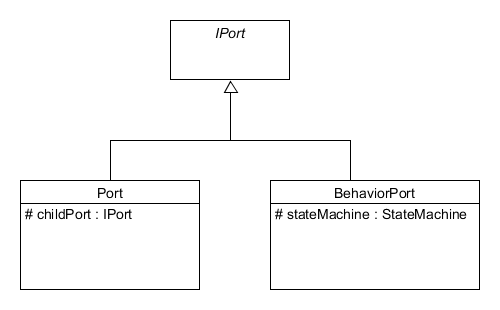
\includegraphics[scale=0.7]{behav_generalport_diag.png} \\
\end{center}
\caption{Különböző típusú portok kezelése leszármazással}
\end{figure}

Az 3.19-es ábrán a két speciális port látható különböző adattagokkal.

\item \textit{Behavior} jelzéssel: \\

\begin{figure}[H]
\begin{center}
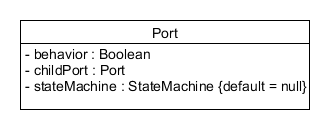
\includegraphics[scale=0.7]{simple_port_diag.png}
\end{center}
\caption{Különböző típusú portok kezelése adattaggal}
\end{figure}

Az 3.20-as ábrán az a megoldás látható, hogy minden adatot egy osztályon belül eltárolunk, és a \textit{behavior} adattag dönti el a port típusát. A másik lehetőség lehetne, hogy az alapján döntünk a típusról, hogy melyik adattag van kitöltve, bevezethetnénk akár egy \textit{Optional} típust is. 

\item \textit{Unio} típussal: \\

\begin{figure}[H]
\begin{center}
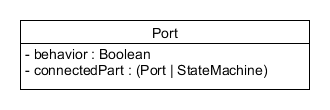
\includegraphics[scale=0.7]{unio_port_diag.png}
\end{center}
\caption{Különböző típusú portok kezelése \textit{unio} típusú adattaggal}
\end{figure}

Itt mindenképpen kell a \textit{behavior} jelző, hogy el tudjuk dönteni, pontosan melyik adattagra hivatkozhatunk az \textit{unio} típusú adattagból. 
\end{enumerate}

\subsection{Konnektorok reprezentálása C++-ban}
A konnektorok reprezentálására is több lehetőségünk van, ezeket fogjuk most megvizsgálni
\begin{enumerate}
\item Itt is felmerül a lehetőség, hogy teljesen figyelmen kívül hagyjuk a konnektorokat. Ezt akkor tehetjük meg a legegyszerűbben, ha a referencia tárolást választjuk a fentiekben az összekapcsolt portok reprezentálásánál. Ennek előnye szintén az egyszerűség lesz, a generált kód mérete kisebb lesz. Hátránya pedig a validáció teljes hiánya, bármilyen két portot összekapcsolhatunk C++-ban. Az interfészeknél arra jutottunk, hogy szükséges a validáció, így ez nem a legjobb megoldás.
\item A másik lehetőségünk bevezetni egy \textit{Connector} osztályt, és összekapcsolásánál erre az osztályra hivatkozunk. Ebben a struktúrában leírhatnánk a portokat, melyek potenciálisan kapcsolódnak egymáshoz, és ezt használhatjuk validációra. Ennek előnye egy tiszta reprezentáció lesz, hátránya viszont az, hogy egy redundáns megoldást kapunk, ha a referenciákat a portokon belül tároljuk, a konnektoroknak semmi szerepük nincsen a validáción kívül,
\item A Konnektorokhoz generált asszociáció típust használjuk fel a validációra. Ennek előnye, hogy az asszociációkat muszáj kigenerálni, függetlenül a konnektoroktól, így nem igényel további strukturális kódgenerálást. Azonban a típusvalidációról gondoskodik, nem enged összekapcsolni olyan két portot, melyhez nem tartozik megfelelő típusú asszociáció. Hátránya, hogy nem elég konkrét, nem kell megfelelni a konkrét szerepeknek a struktúrán belül, elég, ha az interfészeik megfelelnek egymásnak.
\item A legoptimálisabb megoldás most is az utóbbi két megoldás előnyeinek az összekeveréséből lesz. A \ref{conn_cpp} fejezetben megállapítottuk, hogy fordítási időben képesek vagyunk eldönteni egy adott portról, hogy az milyen típusú kapcsolatban állhat a referenciában lévő porttal (assembly vagy delegáció), mivel az UML modellben megtalálhatóak ezek a konnektor struktúrák, melyekből egyértelműen el tudjuk dönteni, potenciálisan milyen kapcsolat jöhet létre a két port között. Ha nem tudnánk eldönteni, egy nem egyértelmű, hibás modellt írnánk, mellyel most nem foglalkozunk. A konnektorból nem csak annak típusát, de a szerepnevet is ki tudjuk nyerni, mely meg fog egyezni a generált asszociáció szerepneveivel. A C++ \textit{Connection} referencia típusában pedig nem csak azt kódolhatjuk bele, milyen típusú kapcsolatban áll az adott porttal, hanem azt is, hogy az átellenes port milyen szereppel van jelen. A referenciák beállítása pedig csak egy olyan típusú \textit{Connectiont} enged beállítani, ami megfelel a port szerepének,  melyet a  port sablonparaméterében adhatunk meg. Ha egy hiányos modellben nincs kapcsolatban egy port egy adott \textit{Connector}-on keresztül senkivel, akkor megadhatnánk egy extremális \textit{NoRole} szerepet, de itt már egyértelműen érdemes sablonspecializációval dolgozni, és a \ref{conn_cpp} fejezetben említett módon egyszerűen használni a \textit{NoConnection}-re specializált verziót.  \\
Előnyök:
\begin{itemize}
\item Továbbra is elég csak asszociációkat generálni a megfelelő szerepekkel.
\item A típus és szerep validációról is gondoskodunk, nem engedünk két olyan portot összekapcsolni, melyek között nincsen \textit{Connector}.
\end{itemize}
Hátrányok:
\begin{itemize}
\item Azonban a portok kódja elbonyolódik sablonparaméterekkel, mely külső kód esetén nem optimális.
\end{itemize}
Példa:
A példában van két portunk (\textit{p1 és p2}), \textit{r1} és \textit{r2} szerepekkel, melyek assembly kapcsolatban állnak egymással (lásd 3.22-es ábra):
\begin{lstlisting}
(p1) r1 <-> (p2) r2
\end{lstlisting}

\begin{figure}[H]
\begin{center}
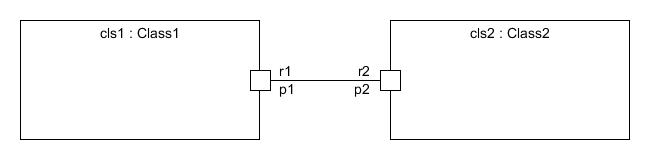
\includegraphics[scale=0.6]{conn_role_comp.png}
\end{center}
\caption{Példa kompozit struktúrája}
\end{figure} 

\begin{figure}[H]
\begin{center}
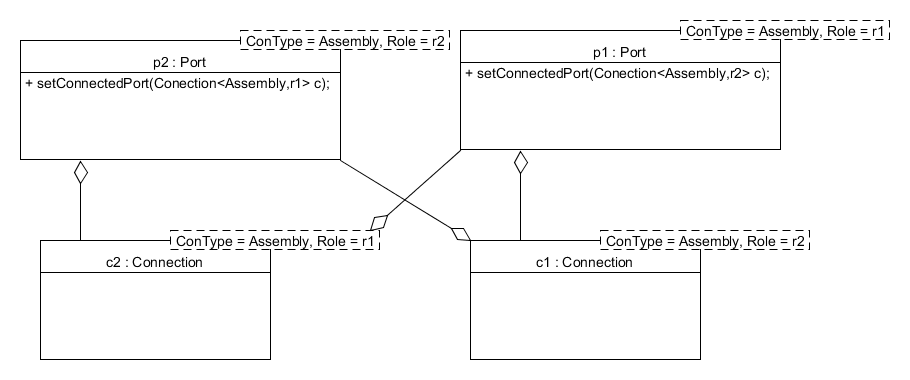
\includegraphics[scale=0.5]{conn_role.png}
\end{center}
\caption{Megoldás objektumdiagramja}
\end{figure}


Ekkor az ábrán azt láthatjuk, hogy a \textit{p1} port - mely a kapcsolatban \textit{r1} szereppel áll - tartalmaz egy kapcsolt portot \textit{r2} szereppel, és fordítva. A \textit{Connection} objektumok pedig értelem szerűen a szerepüknek megfelelő portot tartalmazzák. Amikor pedig beállítjuk a megfelelő kapcsolatot, akkor csak a megfelelő típusú és megfelelő szerepű végpontot adhatjuk meg (a \textit{p1} portnak csak assembly végpontot \textit{r2} szereppel), egyébként pedig fordítási hibát kapnánk. 
\end{enumerate}

\section{Kommunikáció megvalósítása C++-ban} \label{comm}
Végül még érdemes néhány szót ejteni a kommunikációs szemantikáról. Ennek nagy részét már tisztáztuk. Megvizsgáltuk a portra való üzenetküldés szemantikáját az osztályon belülről. Ekkor az üzenetet kifele továbbítjuk, egy másik port fogja megkapni. Ebben a fejezetben csak az lesz az érdekes, hogy az üzenet továbbítások végén, amikor eljut az üzenet egy állapotgéphez, hogyan fogjuk feldolgozni. Így csak az állapotgéppel összekapcsolt portok fogadó (\textit{receive}) műveletei lesznek érdekesek számunkra ebben a fejezetben. A port tartalmaz egy referenciát az állapotgépre, így tudja neki továbbítani az üzenetet. A \ref{cpp_gen_port} fejezetben láttuk, hogy a portokkal való kommunikációt hasonlóan fogjuk kezelni, mint ahogy eddig az üzenetküldést kezeltük, tehát továbbítjuk az üzenetet az állapotgép felé. Azonban a nyers továbbítás kevés lenne, mivel egy objektum állapotgépe egy adott porton történő állapotváltozásra kell reagáljon. Így az üzenet feldolgozásakor tisztában kell lennünk azzal, melyik porttól kaptuk meg az üzenetet. Az UML szabványban egy adott átmenetnél felsorolhatjuk az üzenet lehetséges forrásportjait. \textit{txtUML}-ben csak egy portot adhatunk meg, vagy jelezhetjük, hogy az adott üzenet bárhonnan érkezhet, porton kívülről is, vagy bármely portról  (\textit{AnyPort} extremális érték). Ennek megfelelően a meglévő állapot-átmenet táblát érdemes kibővíteni egy új dimenzióval: Megadni, hogy az átmenetben szereplő üzenetnek mely portok lehetnek a forrásai. \\
Eddig \textit{(esemény,állapot)} kulcsú táblánk volt, melynek értékei ez alapján megadták, melyik átmenetnek kell végrehajtódnia. Ennek részletezésével egy korábbi diplomamunka foglalkozik\cite{hack_dip}. Most vizsgáljuk meg, hogyan tudjuk kiterjeszteni ezt a táblát.
\begin{enumerate}
\item A kulcsait kibővítjük egy port típusinformációval, így \textit{(állapot,esemény,port)} hármasokat fog tartalmazni az átmenet táblánk. Mielőtt egy port továbbítja az állapotgépnek az üzenetet, beállítja az eseményen a port infót, így tudni fogjuk, ki a forrás portja. Ez a \textit{txtUML} esetében jól fog működni, mivel csak egyféle portról jöhet az üzenet. Azonban, ha azt adjuk meg, hogy bármelyik portról érkezhet az üzenet, már problémákba ütközünk, mivel ilyenkor nincs megadva port dimenzió a táblában, az üzenetben viszont igen. Ezt speciálisan le tudjuk kezelni az üzenetfeldolgozás során, azonban ez nem egy elég általános megoldás. \\

\begin{figure}[H]
\begin{center}
\begin{tabular}{@{}ccc|c@{}} \toprule
\multicolumn{4}{c}{Átmenet tábla} \\\midrule
Esemény & Állapot 	& Port 	& Átmenet-Őrfeltétel\\\midrule
Event1 	& State1 	& Port1 & Ttransition1-Guard1 \\
... 	& ... 		& ... 	& ... \\
EventN 	& StateN 	& PortN & TtransitionN-GuardN
\end{tabular}
\small
\caption{Port dimenzióval kiegészített ábra}
\end{center}
\end{figure}

\item Általánosabb megoldás, ha a port helyett megadhatnánk egy maszkban azokat a portokat, melyek lehetséges forrásai lehetnek egy átmenetnek. Mivel egy üzenet továbbra is csak egy helyről érkezhet, így elég lenne csak azt vizsgálnunk, hogy az \textit{(állapot,esemény)} kulcs alapján megkeresett átmenet érték portjai között szerepel-e a az a port, melyről az üzenet érkezett. Itt a port dimenzió a táblázat értékei között jelenik meg. A táblából, hasonlóan az eddigiekhez, \textit{(állapot,esemény)} pár alapján keresünk, melyből megkapjuk az átmenet függvénymutatót, az őrfeltételt, valamint a megfigyelt portokat. Ekkor azt az átmenetet hajtjuk végre, melynek forrásportjai között szerepel az üzenet forrásportja. Azt az esetet, amikor egy üzenet forrása nem port, egy extremális \textit{NoPort} speciális értékkel jelezhetjük. \textit{AnyPort} esetén az osztály összes lehetséges portját belerakjuk az átmenetbe, valamint a \textit{NoPort} típust is. \\

\begin{figure}[H]
\begin{center}
\begin{tabular}{@{}cc|c@{}} \toprule
\multicolumn{3}{c}{Átmenet tábla} \\\midrule
Esemény & Állapot 	&  Átmenet-Őrfeltétel-Portok\\\midrule
Event1 	& State1 	&  Ttransition1-Guard1-Ports1 \\
... 	& ... 	 	& ... \\
EventN 	& StateN 	& Ttransition1-Guard1-PortsN
\end{tabular}
\small
\caption{Port maszkkal kiegészített tábla}
\end{center}
\end{figure}

\end{enumerate}

\chapter*{4. Portok felhasználása a modellezésben}
\stepcounter{chapter}

\section{FMU modellek generálása}
A portok alapvetően a környezettől való szeparáció igénye miatt jöttek létre, mely elősegíti a komponens-alapú fejlesztést. Ebben a világban egy komponens bármilyen komplexitású lehet, akár az egész modellt tekinthetjük egy komponensnek, melynek van egy belső működése, és portokon keresztül kommunikál a külvilággal, hozzáköthetünk más, hasonló elven felépített modelleket. Ennek az elképzelésnek egy szabványa az FMI (Functional Mockup Interface) \cite{fmi_standard}, mely kommunikációs interfészt ír le funkcionális egységek, modellek között. Ezeket nevezzük FMU-nak (Functional Mockup Unit), mely alatt egy olyan egységet értünk, mely az FMI  szabvány segítségével tud kommunikálni a külvilággal, illetve más egységekkel. Az FMU funkcionalitása leírható egy diszkrét modellként állapotgéppel, mely input adatok hatására megváltoztatja a belső állapotát. Az FMI szabvány rendelkezik a \textit{DoStep} művelettel, melyben megadjuk az aktuális input adatokat, és végrehajtjuk a megfelelő állapotváltozást. Ezek olyan folytonos modellekkel vannak összekötve, melyek logikáját differenciálegyenletekkel lehet leírni, melyek folyamatosan mérik a külvilág állapotváltozását (pl. egy fűtésrendszernél, hogy mennyi a hőmérséklet és egyéb külső tényezőket), ezeket adott időközönként továbbítják egy FMU-nak a \textit{DoStep} műveleten keresztül, mely megfelelően reagál a változásra (pl. abbahagyja a radiátortest melegítését). Ezek kommunikációja nem triviális, felmerül például az a kérdés, hogy milyen időközönként kapjon inputot a diszkrét modell, amikor a külső tényezők változása általában nem lineáris. (pl. ha egyre nagyobb ütemben változik a hőmérséklet egy kabinban, lehet, túl későn reagálunk az állapotváltozásra, mely emberéletekbe kerülhet.) \\ A portok, interfészek az \textit{OpenCPS}\cite{opencps} nemzetközi projektben is hasznosnak bizonyultak, melyben a \textit{txtUML} segítségével írtunk meg egy \textit{FMU} diszkrét modellt, majd generáltunk belőle a szabványnak megfelelő \textit{C++} kódot, így a modellt össze lehet kötni más modellekkel. Az \textit{FMI} egy \textit{C}-ben írt szabvány, így a \textit{C++} által generált modell összecsomagolható egy FMU-vá. \cite{fmu_export} \\
Ezt az alábbi módon valósíthatjuk meg: létrehozunk egy \textit{FMUEnvironment} külső osztályt, mely implementálja az \textit{FMI} szabványt. A környezetet egy asszociáció segítségével hozzáköthetjük a modellünk egy osztályához,  melynek el tudja küldeni az input adatokat feldolgozásra, és megkapja tőle az output adatokat. Ehhez az \textit{FMUEnvironment}-nek ismernie kell a modellben egy osztályt, mellyel összekapcsoljuk, és az osztálynak is ismernie kell az \textit{FMUEnvironment}-et.   \\
Az asszociáció helyett azonban portokkal is dolgozhatunk. Egy \textit{FMU}-t felfoghatunk egy olyan strukturális rendszernek, melynek két eleme van:
\begin{enumerate}
\item Az \textit{FMUEnvironment}, mely megvalósítja az FMI-t. (pl. a\textit{DoStep} műveletet)
\item Az FMU működését leíró \textit{txtUML} modell.
\end{enumerate}
Ezek után a környezetet és a modellt egy assembly kapcsolat segítségével összekötjük. Így a környezetnek nem kell ismernie a speciális kontroll osztályt, mellyel asszociációban van, de még a modell-re sem kell referenciát birtokolnia, csak a saját portját kell ismernie. A modell osztály pedig az input üzenetet tetszőleges gyerekének delegálhatja, az előzőekben említett kontroll osztálynak is. Az összekapcsolásokat pedig a legfelső osztály végzi el, mely összefogja az egész rendszert. Elég ennek az egy szereplőnek ismernie a modellt és a környezetet.  \\

\subsubsection{Szemléltetve az egyes megoldásokat}


\begin{figure}[H]
\begin{center}
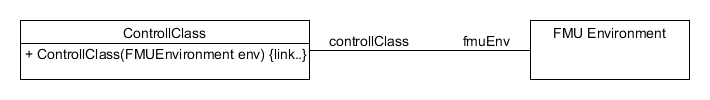
\includegraphics[scale=0.6]{fmu_simple.png} \\
\end{center}
\caption{Asszociációval megvalósított összekapcsolás}
\end{figure}


\begin{figure}[H]
\begin{center}
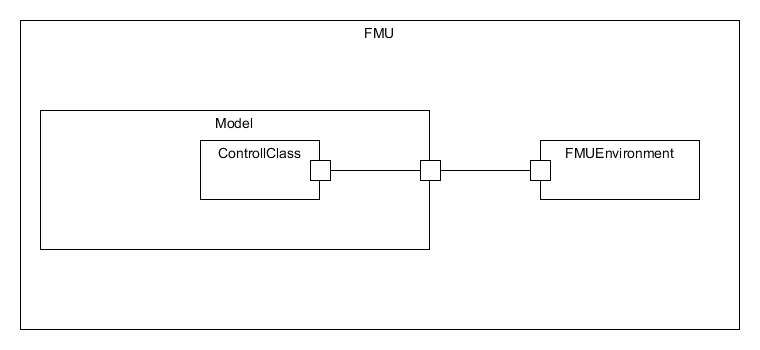
\includegraphics[scale=0.6]{fmu_with_ports.png} \\
\end{center}
\caption{Portokkal megvalósított összekapcsolás}
\end{figure}


Előnyök: \\
\begin{itemize}
\item A modellt függetleníteni tudjuk a környezettől.
\item  Eddig, ha \textit{FMU} kompatibilisen írtuk meg a modellünket, akkor fel kellett venni egy asszociációt, melynek az egyik osztálya az \textit{FMUEnvironment}. Ha ennek ellenére nem szerettünk volna \textit{FMU} generálását, akkor a generált kódban megjelent egy ismeretlen osztályként az \textit{FMUEnvironment} referencia. Mivel az új megoldásban a modell egy olyan egység, aminek csak interfész függőségei vannak a portok révén, így egyszerűen generálhatunk egy forduló modellt akkor is, ha nem szeretnénk \textit{FMU} csomagolást. Ilyenkor elég az interfészeket kigenerálni az \textit{FMUEnvironment} helyett.
\item Tisztább struktúra érhető el, könnyebbé válik bármilyen külső, modelltől független kódot hozzákötni a modellhez. 
\end{itemize}
Hátrányok: \\
\begin{itemize}
\item Nehezebb leírni ezt a strukturális felépítést \textit{txtUML}-ben.
\end{itemize}
Azonban a hátrány kiküszöbölhető azzal, hogy ha a felhasználó beállítja, hogy ha szeretne \textit{FMU}-t generálni a modellből, akkor minden szükséges strukturális kódot legenerálhatunk automatikusan, mivel a modell teljesen függetlenedett az \textit{FMUEnvironment}-től, így azt \textit{txtUML} modellben fel sem kell tüntetni, csak konfigurációnál kell megadnunk, mely portja szolgál majd a külvilággal történő kommunikációra.

\section{Külső szereplők bekötése a modellbe}
Általánosságban elmondható, hogy ha szeretnénk egy külső szereplőt bekötni a modellünkbe anélkül, hogy a generált kódot kézzel meg kéne változtatni (pl. felvenni valamely osztályában referenciaként a külső osztályt), akkor a portok nagy szerepet játszanak ebben. Elég csak felvenni egy csatlakozási pontot a modellben, meghatározni, hogy milyen interfészen keresztül kommunikálhatunk a külvilággal, és kívülről hozzácsatlakozni az adott porthoz. Így, a generált kód teljesen függetlenedik a kézzel írt kódtól, újragenerálás után csak arra kell figyelnünk, hogy a külső kommunikációs port neve ne változzon, az interfésze ne szűküljön. \\

\subsection{Szemléltetve}
\begin{figure}[H]
\begin{center}
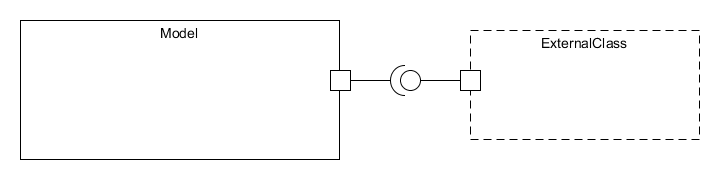
\includegraphics[scale=0.6]{external_with_ports.png} \\
\end{center}
\caption{Külső elemek bekötése a modellbe portokon keresztül}
\end{figure}



\section{Párhuzamosítási lehetőségek kiterjesztése}
A diplomamunkának nem célja a modellekből történő párhuzamos vagy elosztott alkalmazások kódjának generálása. A portok használata azonban egy fontos lépés ezen cél elérésében, mivel portok segítségével úgy tud egymással két osztály kommunikálni, hogy nem tárolnak egymásra referenciát, melynek köszönhetően nem tudnak szinkron hívást kezdeményezni egymás metódusaira, nem tudják elérni egymás publikus adattagjait sem, egyedül aszinkron üzenetküldéssel tudnak kommunikálni egymással. Ennek következtében egy metódus végrehajtásnál egy osztály csak a saját adattagjait olvashatja, írhatja felül, vagy a metódus törzsében létrehozott lokális változókat. Így nem lehet interferencia egy adattag elérésekor akkor sem, ha a portokkal kommunikáló osztályokat külön szálak vagy processzek futtatják. Ehhez arra is szükségünk van, hogy egy szignál ne tartalmazzon referencia értékéket, csak lemásolt, vagy primitív objektumokat. Továbbá statikus függvényhívásokra és változóelérésekre sem szabad lehetőséget adni az egyes osztályoknak, vagy ezen eléréseket szinkronizálni kell. \\

Ezen primitív szabályokat betartva elmondható, hogy két azonos szinten lévő, assembly kapcsolattal kommunikáló osztály porton keresztül kommunikálva nem fog interferenciába keveredni egymással. Szülő-gyerek kapcsolat esetén azonban nem ilyen szerencsés a helyzet, mivel a szülő kompozícióban áll a gyerekével, így referenciát tárol rá a szabvány szerint. Így ezen osztályok párhuzamosítása egy nehezebb feladat, és mivel a párhuzamosítás témája túlmutat a diplomamunka témakörén, így ezt sem vizsgájuk részletsebben.

\section{Testre szabható protokoll}
Egy portra való üzenetküldés megvalósítását tetszőlegesen kicserélhetjük, a \textit{send} művelet megvalósítása akár egy, a modell mellé írt konfigurációtól is függhet. Ha két osztályt szeretnénk különböző szálakra helyezni, akkor valamilyen szálbiztos megvalósítást kell alkalmaznunk. Ha az egész modellünk egy szálon fut, akár valamilyen szinkron hívást is megvalósíthatunk a háttérben. Két osztály akár különböző processzben is futhat, ez esetben a portoknak valamilyen interprocessz kommunikációt kell implementálnia. Ezen lehetőségek részletes elemzése szintén túlmutat a diplomamunka témakörén. 

\section{Az UML szabvány egyszerűbb szemléltetése}
Amikor komponensekről, szereplők izolációjáról, elvárt és szolgáltatott interfészekről, konnektorokról beszélünk az UML kapcsán, akár egy egyetemi előadás keretében, akkor a \textit{txtUML} portjai, annak szemantikájának demonstrálása egy modellen, és C++ megvalósítások elemzése hasznos anyag lehet, hogy a hallgatókhoz közelebb kerüljenek ezek a fogalmak. Így a későbbiekben a rendszerek tervezésénél nem csak egymással asszociációban lévő osztályokban fognak gondolkodni, hanem teljesen izolált szereplőkben is, melyek kommunikációs pontokon, portokon keresztül kommunikálnak a külvilággal. 


\chapter*{5. Megvalósítás}
\stepcounter{chapter}

A dolgozatban nem csak elemeztük a lehetséges megoldásokat, hanem kiválasztottunk egy lehetséges megoldást, melyet leprogramozva demonstrálni tudjuk a dolgozat eredményeit. A továbbiakban ennek a demonstrációs programnak a rövid felhasználói és fejlesztői dokumentációja következik.

\section{Felhasználói interfész tervezés}
A dolgozat a \textit{txtUML} keretrendszerre épül, melynek részletes felhasználói dokumentációja megtalálható annak hivatalosan honlapján \cite{txtuml_web}.

A dolgozat szempontjából a \textit{Portok}, \textit{Interfészek}, \textit{Konnektorok} leírása a legfontosabb, valamint az exportálás és fordítás.

\subsection{Szükséges eszközök}
Az exportáláshoz az alábbi eszközökre van szükségünk:
\begin{itemize}
\item Java
\item Eclipse IDE az exporter dialógus eléréshez, minden szükséges függőség letöltődik a txtUML pluginnal.
\end{itemize}

A fordításhoz az alábbiakra van szükségünk:
\begin{itemize}
\item CMake segítségével legenerálhatjuk a számunkra tetsző fordítási környezetet
\item GCC vagy Clang
\item A generálandó fordítási környezet (MinGW, Ninja, MSVC, stb.).
\end{itemize}

\subsection{Generálás és futtatás}
Kódot generálni legegyszerűbben Eclipse-ből tudunk egy \textit{txtUML} modell megírása és egy kihelyezési konfiguráció alapján. A kódgenerálás eredményeként különféle kódok keletkeznek, különböző szerepekkel, különböző helyeken, melyek két nagy csoportra bonthatók.  A \textit{runtime} mappában az előre megírt fájlokat másoljuk, mely tartalmazzák többek között a \textit{Port} osztályt is, az összekapcsoló műveleteket, és azok szemantikáját. Ezek a kódok keretrendszerként funkcionálnak, minden modellnél megegyeznek. A konkrét port példányokat, konnektorokat, interfészeket pedig a \textit{runtime} mappán kívül generáljuk az input modell alapján. \\

A generált kódot fordítani a \textit{cmake}, valamint a kiválasztott fordítási környezet parancsával tudunk. A \textit{cmake} parancs elhagyható, ha az exporter dialóguson kiválasztjuk a megfelelő környezetet. Fordítás után pedig már futtathatjuk a \textit{main} futtatható állományunkat.

\section{Rendszerarchitektúra}
A program a \textit{txtUML} keretrendszer C++ fordító és exportáló komponensét fejleszti tovább, ennél fogva Java nyelven készült. A Java modellt \textit{JDT} segítségével járjuk be, és az \textit{EMF} keretrendszert használjuk a szabványos modell létrehozásához. \\

\subsection{Szerkezeti felépítés}
A program négy jól elkülöníthető részből áll, mind a négy részt ki kellett egészíteni a \textit{Portok}, \textit{Interfészek}, \textit{Konnektorok} exportáláshoz

\begin{enumerate}
\item A \textit{Java} modellt \textit{UML} modellre leképző algoritmusok. Ezek nem tiszta Java-ban, hanem \textit{Xtend} keretrendszerben készültek. A strukturális elemekhez fel kellett venni a \textbf{PortExporter.xtend}, \textbf{InterfaceExporter.xtend}, \textbf{ConnectorExporter.xtend} és a \textbf{ConnectorEndExporter.xtend} fájlokat. Az akcióelemekhez pedig felvettük a port referenciát kiolvasó \textbf{PortReferenceExporter.xtend} fájlt, az üzenetküldéshez a \textbf{SendToPortActionExporter.xtend}, az összekapcsolásokhoz a \textbf{AssemblyConnect.xtend} valamint a \textbf{DelegateConnect.xtend} fájlokat.
\item Az \textit{UML} modellt feldolgozó algoritmusok. Itt hozzá kellett adni a  \textbf{PortExporter.java} és az \textbf{InterfaceExporter.java} osztályokat, melyek ezek struktúrájának az exportálásáért felelnek. A \textit{send} és a \textit{connect} műveletek exportálása végett hozzá kellett nyúlni az \textbf{ActivityExporter.java} osztályhoz, mely az akciókódok exportálásáért felelős.
\item C++ kódgenerálási sablonok. Itt bevezettük az \textbf{InterfaceTemplates.java} és \textbf{PortTemplates.java} fájlokat a strukturális elemek sablonjához. Az \textbf{AssociationTemplates.java} az összekapcsoláshoz szükséges sablonokról gondoskodik.
\item Előre megírt C++ fájlok. Itt lényegében a \textbf{PortUtils.hpp} fájl tartalmaz minden portokhoz szükséges előre megírt elemet: A portok típusát, a kapcsolatokat, az összekapcsolásokat. Az \textbf{IEvent.hpp}-be is bele kellett nyúlni az eseményfeldolgozás megváltozása miatt. Valamint az \textbf{InterfaceUtils.hpp} tartalmazza az interfészek sablonját és az üres interfészt, a \textbf{AssociationUtils.hpp} pedig az összekapcsoláshoz szükséges asszociációk sablonját.
\end{enumerate}

Ezek a modulok jól elkülöníthetők és cserélhetőek. 

\subsection{Tesztelés}
A demonstrációs program néhány tesztesetét szedjük össze az alábbi fejezetben.

\begin{enumerate}
\item Regresszió tesztelése: Portok nélküli modell létrehozása, melyben azt várjuk, hogy az eredmény maradjon az, ami eddig volt.
\item Egyosztályos modell létrehozása egy darab porttal:
\begin{enumerate}
\item Üres interfészekkel, \textit{send} művelet kipróbálása, mely hibás lesz
\item Nem-üres interfésszel, \textit{send} művelet kipróbálása olyan szignállal, melyet tartalmaz az interfész. Nincs fordítási hiba, de nincs hatása sem. Majd egy olyannal, mely nem része az interfésznek, ekkor fordítási hibát kapunk.
\item Nem-üres interfésszel, állapotgéppel összekapcsolt portot hozunk létre. Az osztály egy átmenete tartalmazza az adott portot. A \textit{receive} művelet kipróbálása megfelelő eseménnyel.
\end{enumerate}
\item Kétosztályos modell létrehozása, egy szülő osztály, melynek van egy belső osztálya. Mindkettőnek van egy-egy portja.
\begin{enumerate}
\item Kompatibilis interfészekkel hozzuk létre őket, delegációval összekapcsoljuk őket, majd \textit{send} művelet kipróbálása a belső osztályon. Ezután a \textit{receive} művelet a külső komponensen.
\item Assembly kapcsolattal összekapcsoljuk őket, mely fordítási hibát jelez.
\item Inkompatibilis interfészekkel hozzuk létre őket, majd delegációval megpróbáljuk összekapcsolni, mely szintén fordítási hibát jelez.
\end{enumerate}
\item Demonstrációs célú modell létrehozása: Egy ping-pong játék struktúra létrehozása, mely tartalmaz egy táblát, valamint egy bírót. Ezek tartalmaznak egy-egy portot, melyek assembly kapcsolattal vannak összekötve. A tábla tartalmaz két játékost, melyek két portot tartalmaznak, egy ping-pong portot, valamint egy olyan portot, melyről a játék kezdése üzenetet várják. A ping-pong portok egymással vannak összekötve, ezen keresztül passzolgatnak egy szignált oda-vissza a játékosok egymás közt, az első játékos pedig delegációval hozzá van kötve a táblához. A játék indulásakor a bíró lead egy játék kezdése szignált a táblának, melyet tovább delegálunk a kezdő játékosnak, és ő elindítja az első szerválást.
\end{enumerate}

A generált kódok megfelelőek, a modellek pedig az elvárt működésnek megfelelően működnek.

\chapter*{6. A diplomamunka eredményei}
\stepcounter{chapter}

Végül foglaljuk össze a diplomamunka főbb eredményeit!
\section{UML kompozíciós szabvány áttekintése, értelmezése}
A kompozíciós elemek az \textit{UML}-nek kevésbé ismert és letisztult részei közé tartoznak, melyet már strukturális szinten is bonyolult értelmezni. A diplomamunka egy alap eszköztárat nyújt a bevezetésben az \textit{UML} kapcsolódó fogalmaira. A portokkal kapcsolatos fogalmakat, az elvárt és szolgáltatott interfészeket, az üzenetküldés és fogadás szemantikáját, portok összekapcsolásáért felelős konnektorokat és konnektor műveletek helyes \textit{UML} reprezentációját és annak szemantikáját mind elemzi a diplomamunka. A helyes leképezés elemzésére a szabványos modell előállításához van szükségünk, míg annak szemantikájára a helyes C++ kód generálásához.

\section{Modellező keretrendszerek, UML szabványok áttekintése}
Az elemzések előtt a diplomamunka megvizsgálja, milyen szabványok segítenek nekünk megtalálni a megfelelő \textit{UML} reprezentációkat az egyes elemekhez, és mi az elemek pontos szemantikája. Majd áttekint különböző modellező keretrendszereket, melyek mindegyike tartalmaz valamilyen kódgenerálást, és megvizsgálja a kompozíciós elemek exportálását. Itt arra jutunk, hogy a legtöbb kertrendszer a kompozíciós elemeket (portokat, konnektorokat) csak nagyon kezdetleges módon támogatja, vagy nem foglalkozik a precíz \textit{UML} szabvánnyal.

\section{C++ fordítási lehetőségek elemzése}
A diplomamunka egyik legfontosabb eredménye a \textit{C++} fordítási lehetőségek elemzése, melyben az \textit{UML} elemek precíz szemantikájának tudatában megvizsgálja, milyen lehetőségek vannak megvalósítani \textit{C++} nyelven a kompozíciós elemeket. Itt a hatékonyságot és a minél tisztább és tömörebb kódot tartjuk szem előtt. A kód tisztaságára azért helyezünk hangsúlyt, mert feltételezzük, hogy a generált kódhoz a felhasználó \textit{C++}-ban ad kiegészítést, integrálva egy meglévő projektbe, felhasználva azt az \textit{API}-t, melyet a generálás során is használhatunk (pl. egy üzenetküldésnél). Az elemzések végén megvizsgáljuk azt is, hogy a kompozíciós modellezés milyen esetben válhat a hasznunkra.

\section{Prototípus készítése a meglévő elemezések alapján}
A diplomamunkához a leírtak alapján implementációt is készítettünk, mely az eredmények demonstrálására, az \textit{UML} szabvány konkrét példákon való megértésére is alkalmas lehet. Továbbá az implementáció segítségével ellenőrizhetjük az elemzéseink helyességét, és hatékonyságát. Az implementációt felhasználva lehetőségünk nyílik átalakítani az \textit{FMU} exportálását is az \textit{OpenCPS} projekt keretein belül.


\chapter*{Köszönetnyilvánítás}
Szeretnénk köszönetet mondani mindazoknak, akik segítettek abban, hogy a diplomamunka létrejöjjön. A \textit{txtUML} egykori és jelenlegi csapatának, akik lefektették a keretrendszer és modellfordító alapjait. Külön köszönet Dévai Gergelynek, aki a \textit{txtUML} ötletgazdája és a diplomamunkám témavezetője volt. Végül szeretnénk köszönetet mondani barátaimnak, családomnak, különösképp nejemnek, akik mellettem voltak egyetemi tanulmányaim során, és támogatták az egyetem elvégzését.


\begin{thebibliography}{4}


\bibitem{uml_omg}
	Object Management Group, 
	\emph{Unified Modeling Language (OMG UML)}, \\
	Standard, Pages 796, December 2017
	\url{https://www.omg.org/spec/UML/About-UML/} November 2018

\bibitem{uml_real}
	Bran Selic, ObjecTime Limited 
	Jim Rumbaugh, Rational Software Corporation,
	\emph{Using UML for Modeling Complex Real-Time Systems}, Article,
	ISBN:3-540-65075-X, 1998, Published in: Proceeding
LCTES '98 Proceedings of the ACM SIGPLAN Workshop on Languages, Compilers, and Tools for Embedded Systems, Pages 250-260  \\
	\url{ftp://ftp.omg.org/pub/umlrtf/UML_rt_ext_F56dist.pdf} November 2018
	
\bibitem{txtUML}
  Gábor Ferenc Kovács, Ádám Ancsin, Gergely Dévai,
  \emph{Textual, executable, translatable UML}, Article, Pages 10,
  14th International Workshop on OCL and Textual Modeling, 2014. 
  \url{http://software.imdea.org/OCL2014/papers/ocl2014_DevaiKA} November 2018
  
  
\bibitem{hack_dip}
	Hack János, 
	\emph{C++ kódgenerálás futtatható UML modellekből}, 
	Thesis, Pages 46, ELTE Informatika Kar, 2015
	
\bibitem{my_szakdolg}
	Nagy András, 
	\emph{Konfigurálható szálkezelés modellfordítóhoz}, 
	Thesis, Pages 50, ELTE Informatika Kar, 2016


\bibitem{alf}
	Object Management Group,
	\emph{Action Language for Foundational UML (ALF)}
	Standard, Version 1.1, Pages 407, June 2017\\
	\url{https://www.omg.org/spec/ALF/About-ALF/} November 2018
	
	
\bibitem{fmul}
	Object Management Group,  \emph{Semantics of a Foundational Subset for Executable UML Models (fUML)} 
	Standard, Version 1.4 beta , November 2018\\
	\url{https://www.omg.org/spec/FUML/About-FUML/} November 2018

\bibitem{pscs}
	Object Management Group, \emph{About the Precise Semantics of UML Composite Structures Specification}, Standard, Version 1.1, Pages 158, March 2018\\
	\url{https://www.omg.org/spec/PSCS/About-PSCS/} November 2018
	
\bibitem{umple}
	Andrew Forward, Omar Badreddin, and Timothy C Lethbridge \\
	\emph{Umple: Towards combining model driven with prototype driven system development}, Article, Pages 7 \\
	In Rapid System Prototyping (RSP), 2010 21st IEEE International Symposium on, pages 1–7. IEEE, 2010.

\bibitem{bridge}
	OneFact, \emph{BridgePoint xtUML tool}, software \\
	\url{http://onefact.net}, November 2018
	
\bibitem{startuml}
	MKLab,  \emph{StartUML}, software, \\
	\url{https://docs.staruml.io/developing-extensions/accessing-elements}, November 2018
	
\bibitem{typelist}
	Codeproject, \emph{TypeLists and a TypeList Toolbox via Variadic Templates}, Atricle,  The Code Project Open License (CPOL), 16 Feb 2016
	\url{https://www.codeproject.com/Articles/1077852/TypeLists-and-a-TypeList-Toolbox-via-Variadic-Temp},
	November 2018
	
\bibitem{fmi_standard}
	Modelica Association, 
	\emph{Functional Mock-up Interface for Model Exchange and Co-Simulation}, 
	Standrad, version 2.0 , Pages 126, , July 25, 2014  \\
	\url{https://fmi-standard.org/docs/2.0.1-develop/}, November 2018
	
\bibitem{fmu_export}
	Jérémie Tatibouet, Ákos Horváth, Zoltán Gera, Boldizsár Nemeth, \\ 
	Dániel Segesdi, Gergely Dévai, Sébastien Revol, \\
	\emph{Interoperability of the standards Modelica-UML-FMI}, Report, Pages 92, Nov 17 2017 \\
	

\bibitem{opencps}
	OpenCPS projekt hivatalos oldala: \\
	\url{https://www.opencps.eu/} November 2018
	
\bibitem{com_book}
  Apperly, H.
  \emph{Service- and Component-based Development Using Select Perspective and UML}, Book, ISBN: 978032115985, Pages 240, Addison-Wesley Professional; 1st edition (January 24, 2003) \\
  \url{https://books.google.com.bn/books?id=k69QAAAAMAAJ} November 2018
  
\bibitem{txtuml_web}
	\emph{txtUML project hivatalos oldala}: \url{http://txtuml.inf.elte.hu/wiki/doku.php} November 2018
	
	
\end{thebibliography}
\end{document}
